% PAKETE UND DOKUMENTKONFIGURATION
\documentclass[11pt, a4paper]{article}

% Encoding für Umlaute
\usepackage[utf8]{inputenc}
\usepackage[T1]{fontenc}

% Silbentrennung
\usepackage[ngerman]{babel}

% erweiterte Matheumgebungen und Formelnummer mit Sectionnummer
\usepackage{amsmath}
\numberwithin{equation}{section}

% Braket Notation
\usepackage{braket}
\usepackage{isotope}
\usepackage[version=3]{mhchem}
\usepackage{chemformula}

% zusätzliche mathematische Schriftarten
\usepackage{amsfonts}

% verschiedene mathematische Symbole
\usepackage{amssymb}

% Einheiten setzen z.B. \SI{10}{\kilo\gram\meter\per\second\squared}
% Fehler: \SI{10 +- 0,2e-4}{\metre}
\usepackage{siunitx}
\sisetup{
  output-decimal-marker={,},
  separate-uncertainty
}

% Einheitendefinitionen
\DeclareSIUnit{\skt}{Skt.}
\DeclareSIUnit{\gauss}{G}
\DeclareSIUnit{\division}{div.}

% Operatordefinitionen
\DeclareMathOperator{\erf}{erf}

% Randbreiten
\usepackage[left=3.5cm,right=3.5cm,top=3cm,bottom=3cm,twoside]{geometry}

% Bilder einfügen
\usepackage{graphicx}

% Verweise innerhalb des Dokuments
\usepackage{hyperref}
\hypersetup{
	colorlinks = true,
	allcolors = {black}
}

% bessere Tabellenlayouts
\usepackage{booktabs}
\usepackage{multirow}
\usepackage{multicol}

% Seitenlayout (Kopfzeile)
\usepackage{fancyhdr}

% Float Barriers
\usepackage{placeins}

% Pakete für gedrehte Subfigures
\usepackage{caption}
\usepackage{subcaption}
\usepackage{rotating}

% Fußnoten in Tabellen - MUSS NACH ROTATING EINGEBUNDEN WERDEN
\usepackage{tablefootnote}

% Paket für textumflossene Abbildungen und Tabellen
\usepackage{wrapfig}

\usepackage{float}

% Caption-Setup
\captionsetup{font={small}}
\renewcommand{\thefigure}{\thesection.\arabic{figure}}
\renewcommand{\thesubfigure}{\alph{subfigure}}
\renewcommand{\thetable}{\thesection.\arabic{table}}
\renewcommand{\thesubtable}{\alph{subtable}}

% Manuelle Silbentrennung
\hyphenation{Sig-nal-ver-hal-ten Szin-til-la-tions-de-tek-tors}

% Tiefe des Inhaltsverzeichnisses (Level: 1 sections, 2 subsections,
% 3 subsubsections)
\setcounter{tocdepth}{3}

% FANCYHDR SETUP
\pagestyle{fancy}
\fancyhead[EL,OR]{\thepage}
\fancyhead[ER]{\leftmark}
\fancyhead[OL]{\rightmark}
\setlength{\headheight}{13.6pt}


\renewcommand{\sectionmark}[1]{
\markboth{\thesection{} #1}{\thesection{} #1}
}
\renewcommand{\subsectionmark}[1]{
\markright{\thesubsection{} #1}
}

\newcommand{\ptt}{Peak-to-Total-Verhältnis}
\newcommand{\co}{\isotope[60]{Co}}
\newcommand{\cs}{\isotope[137]{Cs}}
\newcommand{\eu}{\isotope[152]{Eu}}

% DOKUMENTINFORMATIONEN
\title{P521 \\ Gamma-Spektroskopie mit Szintillations- und Halbleiterdetektoren}

\author{Christopher Deutsch\footnote{christopher.deutsch@uni-bonn.de} \and Christian Bespin\footnote{christian.bespin@uni-bonn.de}}

\date{\today}

\begin{document}

\begin{titlepage}

\maketitle

% DURCHFÜHRUNGSDATUM UND TUTOR
\begin{center}
\begin{tabular}{l r}
Durchführung: & 27./28. April 2015 \\
Gruppe: & $\alpha$ 6 \\
Tutor: & Christian Hammann
\end{tabular}
\end{center}

% ZUSAMMENFASSUNG
\begin{abstract}
\noindent In dem vorliegenden Versuch sollen mit Hilfe eines NaI(Tl) - Szintillationsdetektors und eines Germanium-Halbleiterdetektors Gammaspektren verschiedener Quellen aufgenommen werden.
Diese werden genutzt, um für Detektoren wichtige Größen wie die Peakeffizienz und Energieauflösung zu bestimmen und die beiden genutzten Detektoren hinsichtlich dieser Eigenschaften zu vergleichen. Im Anschluss wird mit dem Halbleiterdetektor eine mitgebrachte Bodenprobe auf Vorkommen von Gammastrahlern hin untersucht.
\end{abstract}

\end{titlepage}

% INHALTSVERZEICHNIS
\tableofcontents
% Neue Seite nach TOC
\newpage

% INHALT VERSUCHSPROTOKOLL
\section{Theorie}

\subsection{Radioaktiver Zerfall}

\subsubsection{Quellen radioaktiver Strahlung}
\label{sssec:quellen_radioaktivität}
Man kategorisiert Quellen radioaktiver Strahlung meistens in \textbf{natürliche Radioaktivität} und \textbf{künstliche Radioaktivität}.
Zu ersterem werden vor allem radioaktive Nuklide gezählt, die bereits seit Entstehung der Erde existieren und heute noch nachweisbar sind (primordiale Nuklide).
Weiterhin werden Nuklide, die bei Zerfällen dieser entstehen sowie kosmische Strahlung der natürlichen Radioaktivität zugeordnet.
Künstliche Radioakivität entsteht gezielt oder als Abfallprodukt bei gesteuerten Prozessen wie der Kernspaltung zur Energiegewinnung oder für medizinische und technische Anwendungen.

\subsubsection{Zerfallsreihen}

Als Zerfallsreihe bezeichnet man eine Kette radioaktiver Zerfälle, bei denen das aus dem zerfallenden Nuklid entstehende Tochternuklid weiter über radioaktiven Zerfall zerfällt.
Von besonderem Interesse sind die natürlichen Zerfallsreihen, die diese Kette radioaktiver Zerfälle für die primordialen Nuklide (s. \ref{sssec:quellen_radioaktivität}) beschreiben.
Es werden hier nur einige der Nuklide aufgeführt, da die Reihen recht lang sind und sich zwischendurch auch verzweigen können (dies geschieht, wenn ein Nuklid in mehrere andere zerfallen kann).
\begin{align*}
	&\isotope[244]{Pu}\to\dots\to\isotope[232]{Th}\to\dots\to\isotope[228]{Th}\to\dots\to\isotope[208]{Pb} &\qquad\text{(Thoriumreihe)}\\
	&\isotope[238]{U}\to\dots\to\isotope[226]{Ra}\to\dots\to\isotope[214]{Pb}\to\dots\to\isotope[206]{Pb} &\qquad\text{(Uran-Radium-Reihe)}\\
	&\isotope[235]{U}\to\dots\to\isotope[227]{Ac}\to\dots\to\isotope[211]{Pb}\to\dots\to\isotope[207]{Pb} &\qquad\text{(Uran-Actinium-Reihe)}
\end{align*}
Die als Thoriumreihe bezeichnete Zerfallsreihe beginnt zwar mit einem Plutoniumnuklid, ist jedoch nach dem am häufigsten auftretenden Element Thorium benannt.
Es existiert darüber hinaus noch eine Neptunium-Reihe ($\isotope[237]{Np}\to\isotope[205]{Tl}$), diese zählt allerdings nicht mehr zu den natürlichen Zerfallsreihen, da das bei Entstehung der Erde vorhandene Neptunium mittlerweile komplett zerfallen ist.
Sie kann nur noch auf künstlichem Weg erzeugt werden, da \isotope[237]{Np} ein Tochternuklid von in Kernreaktoren erzeugten Nukliden ist.

\subsubsection{$\gamma$-Strahlung}

In diesem Versuch wird der atomare Zerfallsprozess mit $\gamma$-Strahlung betrachtet.
Sie entsteht wenn ein energetisch angeregter Atomkern (z.B. nach einem $\alpha$- oder $\beta$-Zerfall) in einen energetisch weniger angeregten Zustand übergeht.
Die dabei frei werdende Energie wird in Form von hochenergetischen Photonen, s.g. Gamma-Quanten ausgesendet, deren Energiebereich von wenigen hundert \si{\kilo\electronvolt} bis zu mehreren \si{\mega\electronvolt} reicht.

\subsection{Wechselwirkung von $\gamma$-Quanten mit Materie}
\label{sec:ww}

Die Wechselwirkung von $\gamma$-Quanten mit Materie kann hauptsächlich auf drei verschiedene Arten erfolgen.
Dabei ist vor allem ihr jeweiliger Wirkungsquerschnitt von Interesse, der angibt, wie die Wechselwirkung der hochenergetischen Photonen von der Energie und Ordnungszahl abhängt.
Ausgehend davon kann beispielsweise festgestellt werden, auf welchen Energiebereichen welche Form der Wechselwirkung dominiert.

\subsubsection{Photoeffekt}
\label{sec:theo_photoeffekt}
Im Bereich niedriger Energie tritt vor allem der Photoeffekt auf.
Dieser beschreibt die Absorption eines Gamma-Quants durch ein atomisches Elektron und kann aufgrund der Impulserhaltung nur im Atom stattfinden.
Bei Einstrahlung eines Photons wird dieses absorbiert und ein Elektron aus dem Atom herausgelöst, dessen kinetische Energie der Energie des Photons abzüglich der Bindungsenergie entspricht.
\begin{align*}
E_\mathrm{kin., e^{-}} = h \nu - E_\mathrm{Bind.}
\end{align*}
Der Wirkungsquerschnitt ist gegeben durch \cite{siegbahn}:
\begin{align*}
	\sigma_\mathrm{Photo.} \propto
	\begin{cases}
		Z^5 E_\gamma^{-\frac{7}{2}} & E_\gamma < m_\mathrm{e} c^2 \\
		Z^5 E_\gamma^{-1} & E_\gamma > m_\mathrm{e} c^2
	\end{cases}
\end{align*}
Insbesondere ist der Wirkungsquerschnitt stark abhängig von der Ordnungszahl $Z$, was eine ausschlaggebende Rolle für die Wahl von Detektormaterialien spielt. Darüber hinaus spiegelt sich die Schalenstruktur des Atoms im Wirkungsquerschnitt wieder, da mit dem Erreichen der Bindungsenergie der nächsthöheren Schale der Wirkungsquerschnitt rapide zunimmt (vgl. Abbildung \ref{fig:photo_total}).

\subsubsection{Compton-Effekt}
\label{sec:compton}
Der Compton-Effekt beschreibt die Streuung von Photonen an freien Elektronen.
Allerdings können Elektronen im Fall $E_\gamma \gg E_\mathrm{Bind. e^{-}}$ auch in Materie als quasifrei betrachtet werden.
Die Streuung beschreibt einen winkelabhängigen Energieübertrag vom Photon auf das Elektron, wobei der Streuwinkel $\theta$ des Photons relativ zur einfallenden Flugrichtung angegeben wird.
\begin{figure}
	\centering
	\includegraphics[width=0.75\textwidth]{./figures/compton.pdf}
	\caption{Streuprozess beim Compton-Effekt}
	\label{fig:comptoneffekt}
\end{figure}
Die Energie des gestreuten Photons $E_\gamma^\prime$ kann aus dem Streuwinkel $\theta$ und der ursprünglichen Energie $E_\gamma$ berechnet werden durch:
\begin{align}
	\frac{E_\gamma^\prime}{E_\gamma} &= \frac{1}{1 + \frac{h \nu}{m_\mathrm{e} c^2} (1-\cos\theta)}
\end{align}
Man sieht, dass die Energie des gestreuten Photons $E_\gamma^\prime$ kontinuierlich bis zu einem Maximalwert bei Rückstreuung ($\theta = \SI{180}{\degree}$) verteilt ist.
Dieser Effekt führt zum Auftreten einer sogenannten Compton-Kante in den aufgenommenen Spektren (vgl. auch \ref{sec:gamma_spektren}).
Die Energie- und Ordnungszahlabhängigkeit des Klein-Nishina-Wirkungsquerschnitt ist gegeben durch \cite{wermes}:
\begin{align}
	\sigma_\mathrm{c} \propto \frac{Z}{E_\gamma}
\end{align}

\subsubsection{Paarbildung}
Die Paarbildung beschreibt die Erzeugung eines Elektron-Positron-Paares aus einem hochenergetischen Photon:
\begin{align}
	\gamma \rightarrow \mathrm{e}^{+} + \mathrm{e}^{-}
\end{align}
Dabei ist $E_\gamma \geq 2 m\mathrm{e} c^2$ durch die Energieerhaltung gefordert.
Der Wirkungsquerschnitt ist gegeben durch \cite{wermes}:
\begin{align}
	\sigma_\mathrm{Paar} \propto Z^2 \ln E_\gamma
\end{align}

\subsubsection{Totaler Wirkungsquerschnitt}
\begin{figure}
	\centering
	\includegraphics[width=0.6\textwidth]{./figures/photocrosssection.png}
	\caption{Summe der Wirkungsquerschnitte für Photoeffekt, Compton-Streuung und Paarbildung in Blei. Quelle: \cite{leo} (modifiziert: Beschriftung hinzugefügt)}
	\label{fig:photo_total}
\end{figure}
Die Summe der in diesem Abschnitt genannten Effekte ergibt sich aus der Summe der einzelnen Wirkungsquerschnitte.
Anhand der genannten Proportionalitäten sieht man bereits, dass für kleine Energien der Photoeffekt ($\sigma_\mathrm{Photo}\propto E_\gamma^{-7/2}$) dominiert.
Im Gegensatz dazu wird die Paarbildung erst bei großen Energien relevant, da deren Wirkungsquerschnitt logarithmisch mit der Gammaenergie zunimmt.
Der Compton-Effekt dominiert in einem Bereich der zwischen dem Dominanzbereich von Photoeffekt und Paarbildung liegt.
Die Summe dieser Effekte wurde in Abbildung \ref{fig:photo_total} für Blei beispielhaft aufgetragen.

\subsection{Detektoren}

\subsubsection{Charakteristische Größen eines Detektors}
\begin{itemize}
	\item \textbf{Energieauflösung:} 
	Die Energieauflösung eines Detektors ist gegeben durch die volle Halbwertsbreite $\Delta E$ der mit ihm aufgenommenen monoenergetischen Linien.
	Die Breite einer solchen Linie wird durch statistische Fluktuationen in der Anzahl der Ionisationen/Anregungen $N$ im Detektormaterial durch das detektierte Teilchen verursacht.
	Die relative Linienbreite geht dabei wie $\mathcal{R} = \Delta E / E \propto 1 / \sqrt{N}$ und nimmt damit mit zunehmenden Ionisationen/Anregungen ab, das heißt die Auflösung nimmt zu.
	
	Aus diesem Grund erreicht der Ge-Halbleiterdetektor eine höheres Auflösungsvermögen, da zur Bildung eines Elektron-Loch-Paares weniger Energie benötigt wird als zur Anregung von Elektronen im Szintillator und dadurch mehr Elektronen-Loch-Paare entstehen.
	Darüber hinaus ist das Auflösungsvermögen eine Funktion der Gammaenergie $E_\gamma$, da hochenergetische Photonen im Detektormaterial mehr Ereignisse $N$ erzeugen als niederenergetische. Wegen $N \propto E_\gamma$ folgt also:
	\begin{align*}
		\mathcal{R} \propto \frac{1}{\sqrt{E_\gamma}}
	\end{align*}
	Das Auflösungsvermögen nimmt demnach mit steigender Energie zu.
	
	Neben dieser intrinsischen Unschärfe des Detektors kommt es noch zu einem weiteren Beitrag durch die verwendete Elektronik, welche sich quadratisch addiert:
	\begin{align*}
		\Delta E^2 = \Delta E_\mathrm{Detektor}^2 + \Delta E_\mathrm{Elektronik}^2
	\end{align*}
	Dieser Zusammenhang wird in Abschnitt \ref{sec:fwhm_halb} experimentell überprüft.
	
	\item \textbf{Absolute Peakeffizienz:}
	Die absolute Peakeffizienz ist definiert durch:
	\begin{align*}
		\mathcal{E} = \frac{\text{Anzahl der Ereignisse im Peak}}{\text{Anzahl der in Richtung des Detektors emittierten Teilchen}}
	\end{align*}
	Wird eine Punktquelle der Aktivität $A$ angenommen, so zerfallen $A\cdot T$ Kerne in einer Zeit $T$.
	Da die Zerfälle isotrop verlaufen, kann der Bruchteil der auf den Detektor einfallenden Teilchen durch Multiplikation mit dem geometrischen Faktor $\frac{\pi r^2}{4 \pi d^2}$ berechnet werden.
	Dabei bezeichnet $r$ den Radius des Detektors und $d$ den Abstand des Detektors von der Quelle.
	Dieser Faktor entspricht gerade dem Bruchteil des Raumwinkels den der Detektor aufspannt und die Anzahl der auf den Detektor einfallenden Teilchen ist gegeben durch:
	\begin{align*}
		A \cdot T \cdot \frac{\pi r^2}{4 \pi d^2}
	\end{align*}
	Schließlich folgt für die absolute Peakeffizienz:
	\begin{align}
		\label{eq:peakeffizienz}
		\mathcal{E}_\mathrm{int} = \frac{N_\mathrm{Peak}}{A \cdot T \cdot \frac{\pi r^2}{4\pi \, d^2}}
	\end{align}
	wobei $N_\mathrm{Peak}$ die Anzahl der im Peak detektierten Ereignisse ist.
\end{itemize}

\subsubsection{Szintillatoren}
Ein Szintillator ist ein Stoff, dessen Atome/Moleküle bei Bestrahlung durch ionisierende Strahlung angeregt werden und folglich Licht emittieren.
In Kombination mit einem Photomultiplier können Szintillatoren als Teilchendetektoren verwendet werden, da das Verhalten von Szintillatoren über einer Mindestenergie linear ist (die Anzahl der erzeugten Photonen ist proportional zur Energie des einfallenden Teilchens).\\
\\
Der in diesem Versuch verwendete Szintillator ist ein NaI-Kristall, welcher mit Tl-Aktivator-Zentren dotiert wurde.
Ein einfallendes Photon löst im Kristall eine Elektronenkaskade aus, welche solange anhält bis die Energie gleichmäßig auf den Elektronen des Kristalls verteilt wurde und die Elektronen eine ausreichend kleine Energie haben um mit den Atomen rekombinieren zu können.
Bei der Rekombination kommt es dabei zur Emission eines Photons, welches umgehend vom Szintillator absorbiert wird, da dieser aufgrund der Bandstruktur im Kristall nicht für die Rekombinations-Photonen transparent ist.
Um ein detektierbares Signal in Form von Photonen im Sichtbaren-/UV-Bereich zu erhalten, wurde der Szintillator mit Thallium dotiert.
Diese Dotierung führt zu zusätzlichen lokale Energieniveaus (Exciton-Band) zwischen dem Leitungsband und dem Valenzband des Kristalls.
Trifft ein Elektronen-Loch-Paar, welches durch ein einfallendes Gamma-Quant im Kristall ausgelöst wurde auf ein solchen Aktivator-Zentrum, kann das Elektron über das zusätzliche Energieniveau mit dem Loch unter Emission von zwei Photonen rekombinieren.
Der Kristall ist aufgrund des geringen Konzentrationsgrades der Dotierung für diese Photonen transparent und kann durch einen Photomultiplier verstärkt werden.

\subsubsection{Halbleiterdetektor}
Ein Halbleiterdetektor funktioniert ähnlich einem Gas-Ionisationsdetektor, wobei anstatt Elektron-Ion-Paaren hier Elektron-Loch-Paare erzeugt werden.
Da Elektron-Loch-Paare aufgrund der geringen Bandlücke bei Halbleitern bei geringeren Energien produziert werden, werden so insgesamt mehr Paare erzeugt, was zu einer hohen Energieschärfe führt.
Durch die im Vergleich zum Gas-Ionisationsdetektor höhere Dichte wird außerdem mehr Energie im Halbleiterdetektor deponiert, was angestrebt wird.
Aufgrund der in einem Halbleiter auftretenden Leckströme (Erzeugung thermischer Elektron-Loch-Paare) ist es notwendig, diesen je nach verwendetem Halbleiter dauerhaft oder nur zur Messung herunterzukühlen (Silizium hat eine relativ große Bandlücke, so dass hier keine Kühlung notwendig ist).
Weitere Störfaktoren sind Oberflächenströme, weswegen der Detektor gut verkapselt werden muss, sowie die Rekombination von Elektronen und Löchern.
Da diese sowohl Energie- und Impulserhaltung erfüllen müssen, geschieht die Rekombination vergleichsweise selten (die Lebenszeiten sind in der Größenordnung Sekunde).
Durch Verunreinigungen im Kristall entstehen allerdings s.g. Rekombinationszentren, die energetisch zwischen Valenz- und Leitungsband des Halbleiters liegen und dort Elektronen einfangen können.
Diese stehen dann nicht mehr zur Messung (Ladungssammlung) zur Verfügung, können allerdings nach einer gewissen Zeit wieder zurück in das Leitungsband gelangen oder aber mit einem ebenfalls eingefangenen Loch rekombinieren.
Ähnlich funktioniert der Effekt des Trappings, welcher auf Verunreinigungen basiert, die nur einen Typ Ladungsträger (Elektron oder Loch) einfangen können und nach einer bestimmten Zeit wieder freigeben.
Aus diesem Grund sind sehr reine Kristalle notwendig, um die Anzahl dieser Rekombinationszentren zu minimieren.\\
\\
Das Signal des Halbleiterdetektors wird als Strom an einem in Sperrrichtung geschalteten pn-Übergang gemessen.
Durch den Übergang zwischen p- und n-Schicht entsteht eine Verarmungszone\footnote{Durch eine zwischen P- und N-Schicht liegende intrinsische Halbleiterschicht kann die Verarmungszone künstlich vergrößert werden.}, in der die Elektron-Loch-Paare durch einfallende Strahlung erzeugt werden.
Das Anlegen einer Spannung in Sperrrichtung bewirkt sowohl eine Vergrößerung der Verarmungszone, in der dann mehr Strahlung detektiert wird und erhöht das elektrische Feld in der Verarmungszone, wodurch eine bessere Ladungssammlung ermöglicht wird.
Die zur Elektron-Loch-Bildung benötigte Energie ist gegeben durch \cite{leo}:
\begin{align}
E_\mathrm{Ge} = \SI{2.96}{eV} \quad \text{für}\quad T = \SI{77}{\kelvin}
\end{align}
Dies ist höher als die Bandlückenenergie, da ein Teil der einfallenden Energie in 
Anregungen des Gitters übergeht.
Im Vergleich zum Szintillationsdetektor ist die Rate für Elektron-Loch-Bildung um zwei Größenordnungen höher, wodurch eine wesentlich bessere Energieauflösung folgt.
Aufgrund der hohen Ordnungszahl von Germanium (verglichen mit Silizium) ist der Wirkungsquerschnitt für den Photoeffekt ca. \num{60} Mal größer, weswegen man zur Gammaspektroskopie Germanium Silizium vorzieht.

\subsection{Gamma-Spektroskopie}

\subsubsection{Photomultiplier}
Ein Photomultiplier dient der gleichzeitigen Messung und Verstärkung eines optischen Signals in Form eines Strompulses.
Ein eintreffendes Photon gelangt auf eine Photokathode und löst dort ein Elektron aus, welches in einem anliegenden Feld zu einer Elektrode hin beschleunigt wird.
Diese Elektrode wird auch als Dynode bezeichnet und ist für die Verstärkung verantwortlich.
Das Elektron erhält durch die Beschleunigung genug Energie, um aus der Dynode mehrere Elektronen auszulösen, wodurch eine Verstärkung erreicht wird.
Schaltet man nun mehrere dieser Beschleunigungsstrecken zwischen zwei Dynoden hintereinander ergibt sich eine mit der Anzahl Dynoden wachsende exponenzielle Verstärkung, wenn das Sekundäremissionsverhältnis (Anzahl der vom eintreffenden Elektron ausgelösten Sekundärelektronen) aller Dynoden gleich ist.
An der letzten Dynode kann dann ein zur Anzahl der ursprünglich einfallenden Photonen proportionaler Strom gemessen werden.

\subsubsection{Vielkanalanalysator}
Zur Beobachtung der am Detektor registrierten Quanten wird ein Vielkanalanalysator verwendet, der über eine festgelegte Anzahl Kanäle verfügt.
Ein im Detektor detektiertes Teilchen einer bestimmten Energie erzeugt einen Strompuls, dessen Ladung proportional zur Energie des Teilchens ist.
In der Regel ist die Linienform dieses Pulses für Teilchen verschiedener Energien gleich, sodass die Impulshöhe ebenfalls eine zur Energie des einfallenden Teilchens proportionale Größe ist.
Ein Vielkanalanalysator kann diese Impulshöhe mit einem Analog-Digital-Wandler messen und dementsprechend die Ereignisse einem Kanal zuordnen.
Dann ist ebenfalls die Kanalnummer proportional zur Energie des detektierten Ereignisses.

\subsubsection{$\gamma$-Spektren}
\label{sec:gamma_spektren}
\begin{figure}[ht]
	\centering
	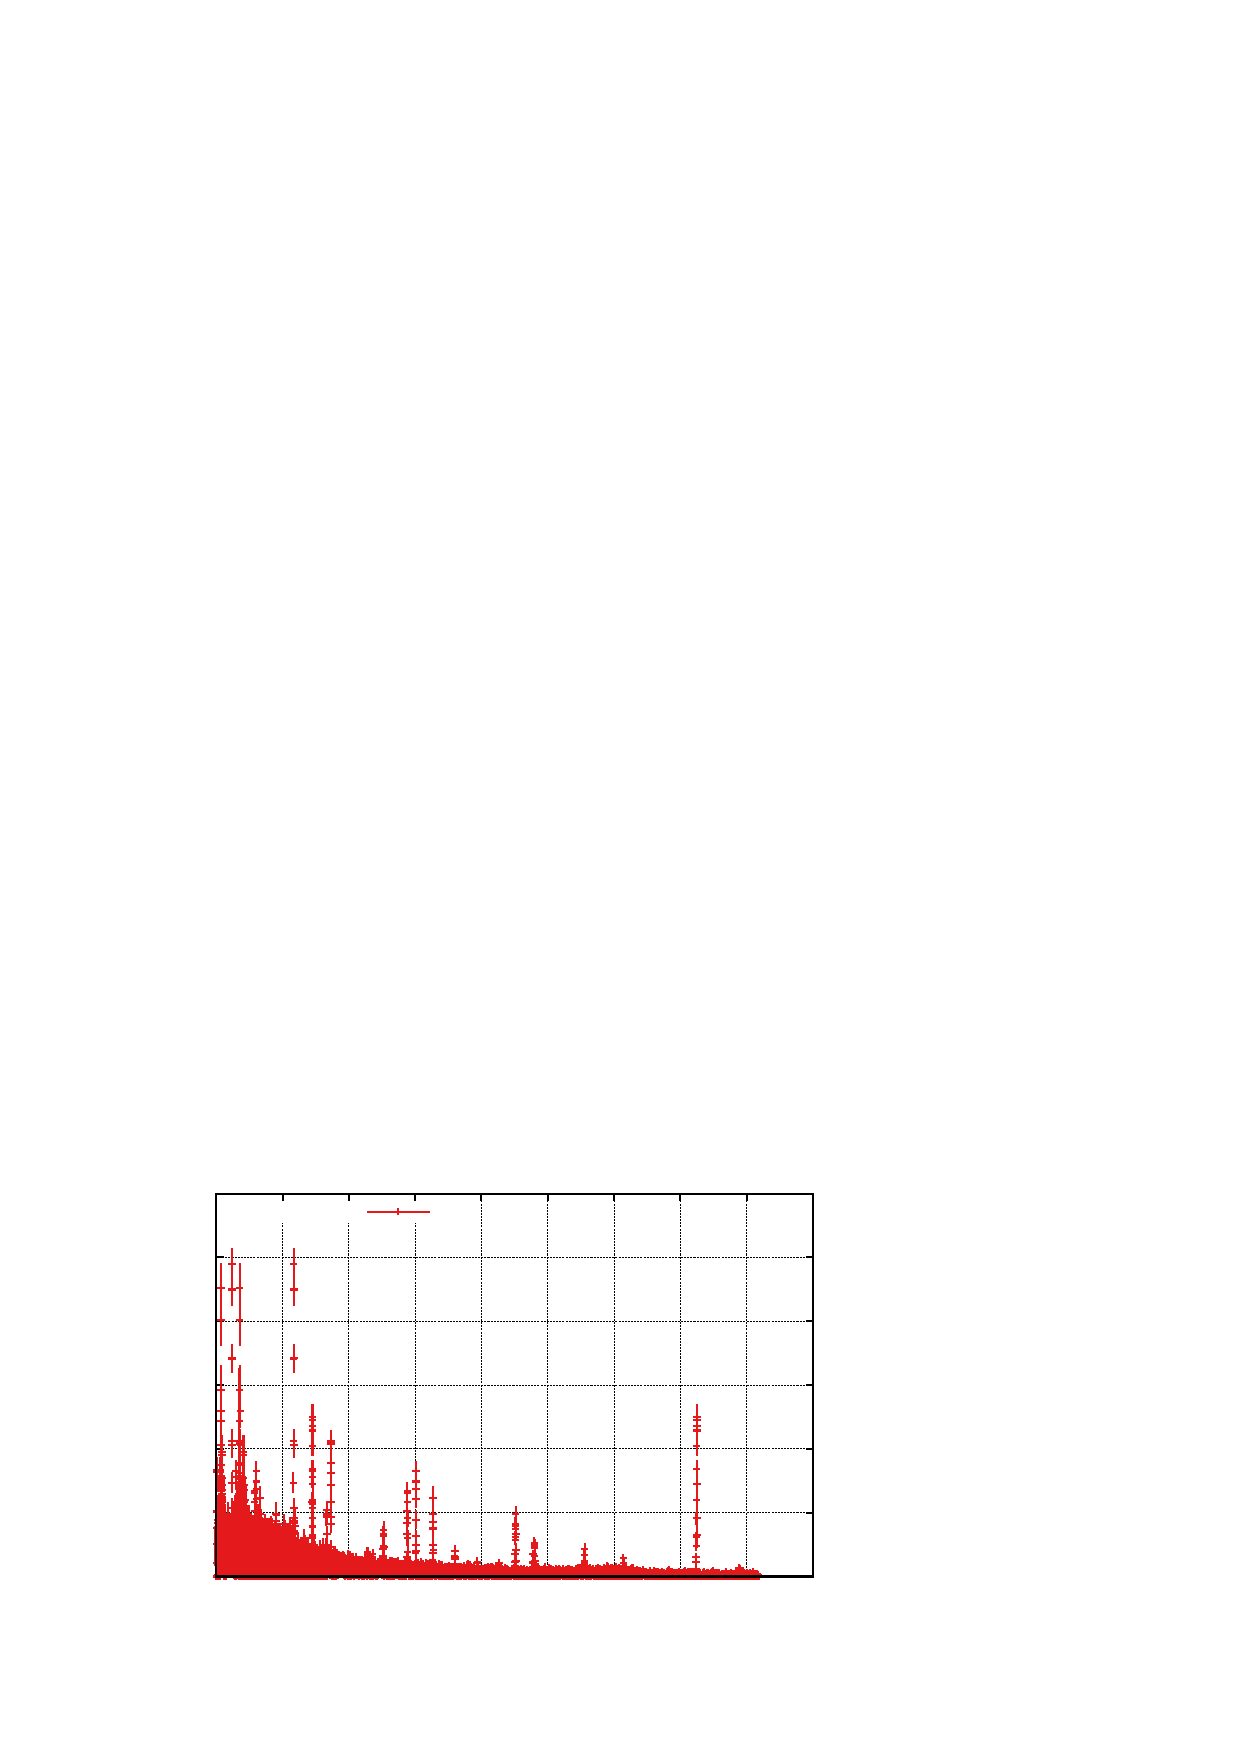
\includegraphics[width=0.8\textwidth]{./figures/spektrum.pdf}
	\caption{Schematische Darstellung von Gamma-Spektren}
	\label{fig:schema_spektrum}
\end{figure}
\noindent Die durch $\gamma$-Spektroskopie aufgenommenen Spektren weisen einige charakteristische Merkmale (Abbildung \ref{fig:schema_spektrum}) auf, die durch die Interaktion von Photonen mit Materie entstehen:
\begin{itemize}
	\item \textbf{Röntgenlinie:}
	Die Röntgenlinie entsteht durch innere Konversion des angeregten Kernes, wodurch die Anregungsenergie auf ein kernnahes Elektron übertragen wird.
	Das Folglich entstandene Loch kann durch Emission eines Röntgenphotons oder eines Auger-Elektrons aufgefüllt werden.
	
	\item \textbf{Rückstreupeak:}
	Der Rückstreupeak entsteht durch Photonen die außerhalb des Detektors z.B. am Detektorgehäuse oder in der Abschirmung durch den Compton-Effekt zurück in den Detektor gestreut werden.
	Dadurch hat das $\gamma$-Quant schon einen Großteil seiner Energie auf das externe Elektron übertragen und kann nach der Rückstreuung in den Detektor mit dementsprechend niedrigerer Energie detektiert werden.
	
	\item \textbf{Escape-Peaks:}
	Sollte die Energie des einfallenden Quants groß genug sein um Paarbildung durchzuführen, so können Elektron-Positron-Paare im Detektormaterial erzeugt werden.
	Diese Paare deponieren ihre gesamte kinetische Energie im Detektormaterial und folglich kann das Positron unter Emission von zwei Photonen mit einem Elektron annihilieren.
	Nun gibt es drei Fälle zu unterscheiden:
	\begin{enumerate}
		\item Beide durch Annihilation entstandenen Photonen verlassen den Detektor ohne weitere Wechselwirkung.
		Dadurch wird nur die kinetische Energie des Elektron-Positron-Paares im Material deponiert und es bildet sich der \textbf{Double-Escape Peak}.
		\begin{align*}
			E = E_\mathrm{kin.}
		\end{align*}
		
		\item Eines der entstandenen Photonen mit $E_\gamma = \SI{511}{keV}$ interagiert mit dem Detektormaterial durch den Photoeffekt und deponiert seine gesamte Energie im Detektor.
		Es kommt zur Ausbildung des \textbf{Single-Escape Peaks}.
		\begin{align*}
			E = E_\mathrm{kin.} + \SI{511}{keV}
		\end{align*}
		
		\item Beide Photonen werden im Detektormaterial absorbiert, wodurch die gesamte Energie des eingefallenen $\gamma$-Quants im Detektor deponiert wird.
		Die Energie eines solchen Ereignisses fällt folglich in den Photopeak:
		\begin{align*}
			E = E_\mathrm{kin.} + 2 \times \SI{511}{keV} = E_\gamma
		\end{align*}
	\end{enumerate}
	
	\item \textbf{Compton-Kante und Kontinuum:}
	In Abschnitt \ref{sec:compton} wurde bereits erwähnt, dass der Energieübertrag durch den Compton-Effekt eine kontinuierliche Energieverteilung mit einer Maximalenergie aufweist.
	Diese ensteht durch die verschiedenen Streuwinkel bei Interaktionsprozessen.
	In den Spektren ist dies als Kontinuum bis zur Maximalenergie sichtbar.
	Dadurch können keine Ereignisse über dem maximalen Energieübertrag durch einmalige Compton-Streuung entstehen und es bildet sich im Spektrum eine charakteristische Kante aus.	
	
	\item \textbf{Photopeak:}
	Der Photopeak im wesentlichen durch die Interaktion der einfallenden $\gamma$-Quanten mit dem Detektormaterial durch den Photoeffekt.
	Dabei wird die gesamte Energie des Photons in dem Detektormaterial deponiert, was dazu führt, dass die Position des Peaks mit der Energie des einfallenden Quants korrespondiert.
	
\end{itemize}

\section{Versuchsaufbau}

Der schematische Aufbau ist in Abbildung \ref{fig:aufbau} dargestellt.
Dabei ist zu beachten, dass der Halbleiterdetektor während der Nutzung gekühlt werden muss, um Leckströme zu verhindern.
\begin{figure}[ht]
	\centering
	\begin{subfigure}{\textwidth}
		\includegraphics[width=\textwidth]{./figures/aufbau_szinti.pdf}
		\caption{Versuchsaufbau mit dem NaI(Tl)-Szintillationsdetektor}	
	\end{subfigure}
	\begin{subfigure}{\textwidth}
		\vspace{20pt}
		\includegraphics[width=\textwidth]{./figures/aufbau_halb.pdf}
		\caption{Versuchsaufbau mit dem Germanium Halbleiterdetektor}	
	\end{subfigure}
	\caption{Schematischer Versuchsaufbau für die beiden verwendeten Detektoren}
	\label{fig:aufbau}
\end{figure}
Bei beiden Detektoren wird das registrierte Signal durch eine Verkettung zweier Verstärker (im Fall des Szintillators durch einen Photomultiplier und anschließenden Hauptverstärker) in den Vielkanalanalysator eingespeist.
Die Verstärker erlauben eine Einstellung der Verstärkung so, dass der gesamte Kanalbereich des Vielkanalanalysators (\num{8192} Kanäle) zur Aufnahme eines Impulshöhenspektrums genutzt werden kann.
Dieses kann am PC direkt betrachtet und zur späteren Auswertung gespeichert werden.
\newpage

\section{Durchführung und Auswertung}
Die ausführliche Durchführung ist der Versuchsanleitung \cite{anleitung} zu entnehmen.
Sollten Abweichungen bei der Durchführung auftreten, so werden diese im jeweiligen Unterkapitel dargestellt.

\subsection{NaI(Tl) Szintillationsspektrometer}
Es wird der Detektor mit Durchmesser \SI{48}{mm} verwendet.


\subsubsection{Detektorsignal des Szintillationsdetektors}
\label{sec:detektorsignal_szinti}
In diesem Abschnitt soll das Signalverhalten des verwendeten NaI(Tl) - Szintillationsdetektors untersucht werden.
Dazu wurden mit einem Oszilloskop die Signalformen jeweils am Vorverstärker des Photomultipliers sowie am Hauptverstärker aufgenommen.
In Abbildung \ref{fig:signal_szinti_vor} ist ein beispielhaftes Signal direkt am Vorverstärker dargestellt.
\begin{figure}[ht]
	\centering
	\begin{subfigure}[b]{0.7\textwidth}
		\centering
		\includegraphics[width=0.7\textwidth]{./figures/signale/vor_szinti_abgeschnitten.jpg}
		\caption{Am Ausgang des Vorverstärkers des Photomultipliers. Die eingestellten Skalenfaktoren am Oszilloskop betragen \SI{0.5}{\volt\per\division} für die Vertikale und \SI{100}{\micro\second\per\division} in der Horizontalen.}
		\label{fig:signal_szinti_vor}
	\end{subfigure}
	
	\begin{subfigure}[b]{0.7\textwidth}
		\centering
		\includegraphics[width=0.7\textwidth]{./figures/signale/haupt_szinti_abgeschnitten.jpg}
		\caption{Am Ausgang des Hauptverstärkers. Die eingestellten Skalenfaktoren am Oszilloskop betragen \SI{1}{\volt\per\division} für die Vertikale und \SI{1}{\micro\second\per\division} in der Horizontalen.}
		\label{fig:signal_szinti_haupt}
	\end{subfigure}
	\caption{Signalformen am Szintillationsdetektor. Die horizontalen Linien markieren \SI{0}{\volt}.}
\end{figure}
Die im Folgenden gemessenen Größen wurden mithilfe eines Bildbearbeitungsprogramms direkt an den Aufnahmen des Oszilloskops abgemessen.
Dabei wurden die Fehler auf \SI{0.2}{\division} der jeweiligen Spannungs-/Zeitskala abgeschätzt.
Das Signal am Vorverstärker des Photomultipliers weist einen (im Vergleich zur Signaldauer) instantanen Anstieg (Anstiegszeit $< \SI{5}{\micro\second}$) mit der Signalamplitude $\Delta U = \SI{2.8 +- 0.1}{\volt}$ auf.
Nach diesem Anstieg fällt das Signal exponentiell mit einer Signaldauer\footnote{Als Definition der Signaldauer $\Delta t$ wird dabei die Zeit verwendet, die das Signal benötigt um von \SI{10}{\percent} der Signalamplitude an der ansteigenden Flanke auf \SI{10}{\percent} an der abfallenden Flanke zu gelangen.} von $\Delta t = \SI{395 +- 20}{\micro\second}$ ab.
Der exponentielle Abfall des Signals kann durch den relativ langsamen Abtransport der Ladung im Sekundarelektronenvervielfacher erklärt werden.
Im Vergleich dazu wurde in Abbildung \ref{fig:signal_szinti_haupt} eines der Signale am Hauptverstärker des Detektors dargestellt.
Obwohl der Puls am unipolaren Ausgang des Verstärkers gemessen wurde, kann ein negativer Ausschlag festgestellt werden.
Der negative Impuls ist für die Messung nicht relevant, da dieser bei der Impulshöhenmessung mit dem Vielkanalanalysator keinen Einfluss hat.
Der für die Messung relevante positive Impuls hat eine Amplitude von $\Delta U = \SI{3.4 +- 0.2}{\volt}$ und eine Signaldauer $\Delta t = \SI{2.3 +- 0.2}{\micro\second}$.
Der Vergleich der Amplituden\footnote{Ein direkter Vergleich der beiden Signale macht nur Sinn, wenn lediglich Größenordnungen betrachtet werden, da die beiden Signale von unabhängigen Ereignissen stammen.} an beiden Verstärkern legt nahe, dass der Hauptverstärker nicht zur Verstärkung der Spannung dient sondern vielmehr zur Impulsformung.
Dies sieht man besonders an der um zwei Größenordnungen verkürzten Signaldauer.
Da beide Signale von unabhängigen Ereignissen stammen, kann leider nicht verifiziert werden, dass die Impulshöhe am Hauptverstärker proportional zur im Photomultiplier gelösten Ladung, ist, welche wiederum proportional zur Fläche über dem Signal am Vorverstärker ist.

\subsubsection{Aufnahme der Gammaspektren von \ch{^{60}Co}, \ch{^{137}Cs}, \ch{^{152}Eu} und des Untergrundspektrums}
Nachdem die Signale des Szintillationsdetektors betrachtet wurden, kann mit der Aufnahme der Spektren begonnen werden.
Dazu muss die Verstärkung des Hauptverstärkers geeignet eingestellt werden, um den Kanalbereich des Vielkanalanalysators optimal auszunutzen.
Dies wird dadurch erreicht, dass die hochenergetische \SI{1408}{keV}-Linie von \isotope[152]{Eu} über die Verstärkung so positioniert wird, dass diese in den Bereich um Kanal 7000 fällt.
Anschließend wird ein Untergrundspektrum aufgenommen, um die Spektren der Isotope \isotope[60]{Co}, \isotope[137]{Cs} und \isotope[152]{Eu} vom Untergrund bereinigen zu können.
Die Messzeit beträgt für alle Spektrenaufnahmen \SI{720}{\second}.
Generell wird für den Fehler auf die Anzahl der Ereignisse $N$ in einem bestimmten Kanal $n$ des Vielkanalanalysators wegen der zugrundeliegenden Poisson-Verteilung:
\begin{align}
\label{eq:poisson_fehler}
\Delta N = \sqrt{N}
\end{align}
angenommen.
Die Untergrundkorrektur erfolgt dann durch Subtraktion des Untergrundspektrums von den aufgenommenen Spektren der Isotope:
\begin{align}
	\label{eq:untergrundkorr_fehler}
	N_\mathrm{korr.} &= N - N_\mathrm{Untergrund}  \nonumber\\
	\Delta N_\mathrm{korr.} &= \sqrt{\Delta N^2 + \Delta N_\mathrm{Untergrund}^2} = \sqrt{N + N_\mathrm{Untergrund}}
\end{align}
wobei der Fehler aufgrund von Gleichung \ref{eq:poisson_fehler} und Gauß'scher Fehlerfortpflanzung folgt.
Aus Gründen der Übersichtlichkeit wurde in Abbildung \ref{fig:abzug_untergrund} der Abzug des Untergrundes am Beispiel der Messung von \isotope[60]{Co} durchgeführt und im Anhang nur noch die vom Untergrund bereinigten Spektren abgebildet.
\begin{figure}[hp]
	\centering
	\begin{subfigure}[b]{0.65\textwidth}
		\resizebox{!}{0.282\textheight}{
		\input{./plots/szintillator/untergrund.tex}
		}
		\caption{Untergrund des NaI(Tl)-Szintillationsdetektors}
		\label{fig:untergrund_szinti}
	\end{subfigure}
	
	\begin{subfigure}[b]{0.65\textwidth}
		\resizebox{!}{0.282\textheight}{
		\input{./plots/szintillator/cobalt_mit_untergrund.tex}
		}
		\caption{Untergrundbehaftetes \isotope[60]{Co}-Spektrum}
		\label{fig:cobalt_mit_untergrund}
	\end{subfigure}
	
	\begin{subfigure}[b]{0.65\textwidth}
		\resizebox{!}{0.282\textheight}{
		\input{./plots/szintillator/cobalt_darstellung.tex}
		}
		\caption{\isotope[60]{Co}-Spektrum mit subtrahiertem Untergrund}
		\label{fig:cobalt_ohne_untergrund}
	\end{subfigure}
	\caption{Subtraktion des gemessenen Untergrundes von dem \isotope[60]{Co}-Spektrum. Die Spektren wurden mit einer Messdauer von $t = \SI{720}{\second}$ aufgenommen. Die Korrektur ist hauptsächlich in den Kanälen $< 1000$ zu erkennen.}
	\label{fig:abzug_untergrund}
\end{figure}
Im Folgenden werden (sofern nicht anders angegeben) alle Spektren gemäß dieser Überlegungen korrigiert, weshalb die korrigierten Ereignisanzahlen ab sofort mit $N$ bezeichnet werden.
Für die Bestimmung der absoluten Peakeffizienz in Abschnitt \ref{sec:absolute_peakeffizienz_szinti} ist der Abstand der radioaktiven Probe vom Detektor nötig, welcher in Tabelle \ref{tab:abstand_szinti} aufgetragen wurde.
\begin{table}[ht]
	\centering
	\input{./tables/abstaende_szintillator.tex}
	\caption{Abstände $d$ der Proben vom Szintillationsdetektors}
	\label{tab:abstand_szinti}
\end{table}

\subsubsection{Energiekalibrierung}
\label{sec:kalibrierung_szinti}
Da die Spektren mit einem Vielkanalanalysator aufgenommen werden, kann aus den Daten zunächst keine Energieinformation gewonnen werden.
Dazu ist eine Energiekalibrierung nötig, die mit Hilfe bekannter Linien in den jeweiligen Gamma-Spektren durchgeführt wird.
An gut getrennte Linien wurde dazu eine Gaußfunktion der Form
\begin{align}
\mathcal{G}(n) &= A \cdot \exp\left( - \frac{(n - \mu)^2}{2 \sigma^2}\right) \qquad\text{($n$: Kanalnummer),}
\label{eq:gaussfithypothese}
\end{align}
im Fall nah beieinander liegender Linien eine Summe von solchen Gaußfunktionen angepasst.
Weiterhin wurde in der Anpassungshypothese ein Untergrund $u(n)$ berücksichtigt, der je nach Peak auf Basis der Daten entweder konstant oder linear angenommen wurde.
Zur Verdeutlichung wurde die Anpassung für Cobalt in Abbildung \ref{fig:fit_cobalt} beispielhaft für das Vorgehen dargestellt.
\begin{figure}[ht]
	\centering
	\resizebox{0.85\textwidth}{!}{
	\input{./plots/szintillator/energiekalibrierung/cobalt_darstellung.tex}
	}
	\caption{Anpassung für die Linien im Gammaspektrum von Cobalt. $\Sigma$ bezeichnet die Summe der beiden Gaußfunktionen $\mathcal{G}$ und des Untergrundes $u$.}
	\label{fig:fit_cobalt}
\end{figure}
In Tabelle \ref{tab:kalibrierungslinien_szinti} sind die Ergebnisse der Anpassung eingetragen, wobei für die Kalibrierung zunächst nur der Linienschwerpunkt $n$ und die Gammaenergie $E_\gamma$ relevant sind.
Den Schwerpunkten der Gaußfunktionen wurden dabei unter Benutzung der Termschemata und Tabelle in \cite{anleitung} die jeweiligen Gammaenergien zugeordnet.
\begin{table}[ht]
	\centering
	\begin{tabular}{lSSSSSSS}
\toprule
Isotop & {Gammaenergie} & \multicolumn{2}{c}{Ampltiude} & \multicolumn{2}{c}{Schwerpunkt} & \multicolumn{2}{c}{Standardabweichung}\\
       & {$E_{\gamma}$ / \si{\kilo\electronvolt}} & {$A$} & {$\Delta A$} & {$n$} & {$\Delta n$} & {$\sigma$} & {$\Delta \sigma$}\\
\midrule
Co & 1173.237 & 780.6     & 4.6    & 6221.1      & 0.4    & 59.4   & 0.4    \\
Co & 1332.501 & 860.1     & 4.9    & 6526.9      & 0.3    & 49.4   & 0.3    \\
Cs & 661.660  & 1062.8    & 6.3    & 3844.1      & 0.6    & 114.3  & 0.6    \\
Eu & 121.783  & 1485.8    & 8.0    & 731.9       & 0.2    & 30.9   & 0.3    \\
Eu & 244.699  & 153.8     & 7.6    & 1421.2      & 2.4    & 45.0   & 2.7    \\
Eu & 344.281  & 403.5     & 3.4    & 1997.5      & 0.5    & 78.9   & 1.0    \\
Eu & 778.903  & 43.2      & 0.9    & 4511.4      & 2.2    & 110.8  & 2.8    \\
Eu & 964.131  & 44.7      & 0.9    & 5535.3      & 1.7    & 100.0  & 2.6    \\
Eu & 1112.116 & 99.5      & 1.4    & 6030.9      & 0.9    & 79.0   & 1.5    \\
Eu & 1408.011 & 93.9      & 1.3    & 6637.7      & 0.7    & 46.4   & 0.8        \\
\bottomrule
\end{tabular}
	\caption{Anpassungsergebnisse zur Energiekalibrierung für den NaI(Tl) Szintillationsdetektor}
	\label{tab:kalibrierungslinien_szinti}
\end{table}
Der Zusammenhang zwischen Kanalnummer und Energie wird als linear betrachtet, so dass eine Anpassung an eine Gerade mit Steigung $m$ und Achsenabschnitt $b$ erfolgt.
Für Kanalnummern über \num{6000} weichen die gefundenen Messwerte deutlich von dem linearen Verlauf der Kanalnummern kleiner als \num{6000} ab, so dass hier nicht die gleiche Kalibrierung verwendet werden kann.
Für diesen Bereich wurde auf Grundlage der dort liegenden \num{4} Datenpunkte eine zweite Kalibrierung (mit gleicher Anpassungshypothese) durchgeführt, so dass im weiteren Verlauf je nach betrachtetem Kanalbereich die dort gültige Kalibrierung gewählt werden muss. 
Die Daten und durchgeführte Anpassung sind in Abbildung \ref{fig:kalibrierung_szinti} zu sehen.
\begin{figure}[ht]
	\centering
	\begin{tabular}{lSSSSSSS}
\toprule
Isotop & {Gammaenergie} & \multicolumn{2}{c}{Ampltiude} & \multicolumn{2}{c}{Schwerpunkt} & \multicolumn{2}{c}{Standardabweichung}\\
       & {$E_{\gamma}$ / \si{\kilo\electronvolt}} & {$A$} & {$\Delta A$} & {$n$} & {$\Delta n$} & {$\sigma$} & {$\Delta \sigma$}\\
\midrule
Co & 1173.237 & 780.6     & 4.6    & 6221.1      & 0.4    & 59.4   & 0.4    \\
Co & 1332.501 & 860.1     & 4.9    & 6526.9      & 0.3    & 49.4   & 0.3    \\
Cs & 661.660  & 1062.8    & 6.3    & 3844.1      & 0.6    & 114.3  & 0.6    \\
Eu & 121.783  & 1485.8    & 8.0    & 731.9       & 0.2    & 30.9   & 0.3    \\
Eu & 244.699  & 153.8     & 7.6    & 1421.2      & 2.4    & 45.0   & 2.7    \\
Eu & 344.281  & 403.5     & 3.4    & 1997.5      & 0.5    & 78.9   & 1.0    \\
Eu & 778.903  & 43.2      & 0.9    & 4511.4      & 2.2    & 110.8  & 2.8    \\
Eu & 964.131  & 44.7      & 0.9    & 5535.3      & 1.7    & 100.0  & 2.6    \\
Eu & 1112.116 & 99.5      & 1.4    & 6030.9      & 0.9    & 79.0   & 1.5    \\
Eu & 1408.011 & 93.9      & 1.3    & 6637.7      & 0.7    & 46.4   & 0.8        \\
\bottomrule
\end{tabular}
	\caption{Energiekalibrierung des NaI(Tl) Detektors. Die Fehler sind zu klein, um gesehen werden zu können.}
	\label{fig:kalibrierung_szinti}
\end{figure}
Die Anpassungsergebnisse lauten:
\begin{align}
	m = 
	\begin{cases}
	\SI{0.17441+-0.00076}{\kilo\electronvolt} & n < 6000 \\
	\SI{0.48976+-0.04034}{\kilo\electronvolt} & n > 6000
	\end{cases}\\
	b = 
	\begin{cases}
	\SI{-5.189+-2.627}{\kilo\electronvolt} & n < 6000 \\
	\SI{-1855.53+-256.50}{\kilo\electronvolt} & n > 6000
	\end{cases}
\end{align}
Da die Anpassungsgerade für den Halbleiterdetektor eine deutlich bessere und durchgehend lineare Übereinstimmung mit den Messwerten zeigt, liegt die Ursache für den beobachteten Verlauf nicht an dem verwendeten Vielkanalanalysator sondern ist im Verstärker zu suchen.\\
\\
Da im Folgenden oftmals eine Umrechnung von Kanalnummer $n$ auf Gammaenergie $E_\gamma$ erfolgt, soll hier die Vorgehensweise einmalig erklärt werden.
Die Kalibrierung bildet den linearen Zusammenhang zwischen $E_\gamma$ und $n$:
\begin{align}
	E_\gamma = m \cdot n + b
\end{align}
Da oftmals die Kanalnummer mit einem Fehler behaftet ist (z.B. bei den Linienschwerpunkten) muss dies bei der Fehlerfortpflanzung:
\begin{align}
	\Delta E_\gamma = \sqrt{n^2 \cdot \Delta m^2 + m^2 \cdot \Delta n^2 + \Delta b^2}
\end{align}
berücksichtigt werden.

\subsubsection{Halbwertsbreiten der Linien}
Zur Bestimmung der Halbwertsbreiten kann die Anpassung der Gaußfunktionen an die jeweilige Linie verwendet werden, welche bereits bei der Energiekalibrierung in Abschnitt \ref{sec:kalibrierung_szinti} durchgeführt werden.
Dazu kann die Standardabweichung $\sigma$ der Gaußfunktion in die volle Halbwertsbreite (FWHM: \textit{full width at half maximum}) durch
\begin{align}
	\text{FWHM} = 2 \, \sqrt{2\ln(2)} \cdot \sigma
\end{align}
umgerechnet werden.
Der Fehler wird dementsprechend durch
\begin{align}
	\Delta \text{FWHM} = 2 \, \sqrt{2\ln(2)} \cdot \Delta \sigma
\end{align}
fortgepflanzt.
Mit den Anpassungsergebnissen aus Tabelle \ref{tab:kalibrierungslinien_szinti} kann dementsprechend die Halbwertsbreite in Einheiten der Kanalnummer berechnet werden.
Diese kann mithilfe der Energiekalibrierung in Abschnitt \ref{sec:kalibrierung_szinti} in Einheiten der Energie umgerechnet werden, wobei die Fehler erneut durch Gauß'sche Fehlerfortpflanzung ermittelt werden.
Konkret erfolgt die Umrechnung durch Multiplikation der Halbwertsbreite in Einheiten der Kanalnummer mit der Steigung der Kalibrierungsgeraden, da die volle Halbwertsbreite eine Differenzgröße ist und dadurch ein konstanter Versatz keinen Einfluss nimmt.
\begin{table}[ht]
	\centering
	\begin{tabular}{lSSSSS}
\toprule
Isotop & {Gammaenergie} & {FWHM} & {$\Delta \text{FWHM}$} & {FWHM} & {$\Delta \text{FWHM}$}\\
       & {$E_\gamma$ / \si{keV}}             & \multicolumn{2}{c}{Kanäle} & \multicolumn{2}{c}{\si{keV}} \\
\midrule
Co            & 1173.237 & 139.8  & 0.9        & 68.5   & 5.7 \\
Co            & 1332.501 & 116.2  & 0.6        & 56.9   & 4.7 \\
Cs            & 661.660  & 269.1  & 1.3        & 46.9   & 0.3 \\
Eu            & 121.783  & 72.8   & 0.6        & 12.7   & 0.2 \\
Eu            & 244.699  & 106.0  & 6.2        & 18.5   & 1.1 \\
Eu            & 344.281  & 185.7  & 2.4        & 32.4   & 0.5 \\
Eu            & 778.903  & 260.9  & 6.6        & 45.5   & 1.2 \\
Eu            & 964.131  & 235.4  & 5.9        & 41.1   & 1.1 \\
Eu            & 1112.116 & 186.0  & 3.5        & 91.1   & 7.7 \\
Eu            & 1408.011 & 109.3  & 1.8        & 53.5   & 4.5 \\
\bottomrule
\end{tabular}
	\caption{Volle Halbwertsbreiten der zur Kalibration verwendeten Linien in den Spektren von \isotope[60]{Co}, \isotope[137]{Cs} und \isotope[152]{Eu}.}
	\label{tab:fwhm_szinti}
\end{table}
Die berechneten Breiten wurden in Tabelle \ref{tab:fwhm_szinti} zusammengetragen.
Leider führt die Nichtlinearität des Verstärkers bei der stückweisen Energiekalibrierung zu einer Verfälschung der Halbwertsbreite der Linien mit einer Energie größer als \SI{1000}{\kilo\electronvolt}, weshalb diese nur als Größenordnungen betrachtet werden sollten.
Die Halbwertsbreiten für Linien geringerer Energie sollten hingegen akkurat wiedergegeben werden.
Betrachtet man nur Linien geringerer Energie so zeigt sich die erwartete Zunahme der Linienbreite mit steigender Energie, welche in dem statistischen Prozess der Photonenemission im Szintillator begründet liegt.

\subsubsection{Peak-to-Total Verhältnis}
\label{sec:ptt_szinti}
Zur Bestimmung des Peak-to-Total Verhältnisses muss die Gesamtzahl aller Ereignisse $N_\mathrm{tot.}$ in den Spektren bestimmt werden.
Diese erhält man durch Subtraktion der Gesamtzahl der Ereignisse der Untergrundmessung $N_\mathrm{Untergrund}$ von der untergrundbehafteten Ereigniszahl des Spektrums $N_0$:
\begin{align}
	N_\mathrm{tot.} = N_\mathrm{0} - N_\mathrm{Untergrund}
\end{align}
Dabei wird auf die Anzahlen der Fehler gemäß der Poisson-Verteilung angenommen.
Neben der Gesamtzahl wird sowohl die Anzahl der Ereignisse in den Photopeaks als auch im Rückstreupeak benötigt.
Diese können direkt durch Integration über die Anpassung der Gaußfunktion berechnet werden:
\begin{align}
\int_{-\infty}^{\infty} \mathcal{G}(n) \, \mathrm{d}n = \sqrt{2 \pi} \sigma A
\label{eq:integral_peak}
\end{align}
Die Anpassungsparameter für die Photopeaks können direkt aus Abschnitt \ref{sec:kalibrierung_szinti} übernommen werden.
Analog zur Kalibrierung wird eine Anpassung an die Rückstreupeaks von \isotope[60]{Co} und \isotope[137]{Cs} durchgeführt.
Exemplarisch dafür wurde die Anpassung an den Rückstreupeak von \isotope[137]{Cs} in Abbildung \ref{fig:fit_rueck_szinti} durchgeführt.
\begin{figure}[ht]
	\centering
	% GNUPLOT: LaTeX picture with Postscript
\begingroup
  \makeatletter
  \providecommand\color[2][]{%
    \GenericError{(gnuplot) \space\space\space\@spaces}{%
      Package color not loaded in conjunction with
      terminal option `colourtext'%
    }{See the gnuplot documentation for explanation.%
    }{Either use 'blacktext' in gnuplot or load the package
      color.sty in LaTeX.}%
    \renewcommand\color[2][]{}%
  }%
  \providecommand\includegraphics[2][]{%
    \GenericError{(gnuplot) \space\space\space\@spaces}{%
      Package graphicx or graphics not loaded%
    }{See the gnuplot documentation for explanation.%
    }{The gnuplot epslatex terminal needs graphicx.sty or graphics.sty.}%
    \renewcommand\includegraphics[2][]{}%
  }%
  \providecommand\rotatebox[2]{#2}%
  \@ifundefined{ifGPcolor}{%
    \newif\ifGPcolor
    \GPcolortrue
  }{}%
  \@ifundefined{ifGPblacktext}{%
    \newif\ifGPblacktext
    \GPblacktexttrue
  }{}%
  % define a \g@addto@macro without @ in the name:
  \let\gplgaddtomacro\g@addto@macro
  % define empty templates for all commands taking text:
  \gdef\gplbacktext{}%
  \gdef\gplfronttext{}%
  \makeatother
  \ifGPblacktext
    % no textcolor at all
    \def\colorrgb#1{}%
    \def\colorgray#1{}%
  \else
    % gray or color?
    \ifGPcolor
      \def\colorrgb#1{\color[rgb]{#1}}%
      \def\colorgray#1{\color[gray]{#1}}%
      \expandafter\def\csname LTw\endcsname{\color{white}}%
      \expandafter\def\csname LTb\endcsname{\color{black}}%
      \expandafter\def\csname LTa\endcsname{\color{black}}%
      \expandafter\def\csname LT0\endcsname{\color[rgb]{1,0,0}}%
      \expandafter\def\csname LT1\endcsname{\color[rgb]{0,1,0}}%
      \expandafter\def\csname LT2\endcsname{\color[rgb]{0,0,1}}%
      \expandafter\def\csname LT3\endcsname{\color[rgb]{1,0,1}}%
      \expandafter\def\csname LT4\endcsname{\color[rgb]{0,1,1}}%
      \expandafter\def\csname LT5\endcsname{\color[rgb]{1,1,0}}%
      \expandafter\def\csname LT6\endcsname{\color[rgb]{0,0,0}}%
      \expandafter\def\csname LT7\endcsname{\color[rgb]{1,0.3,0}}%
      \expandafter\def\csname LT8\endcsname{\color[rgb]{0.5,0.5,0.5}}%
    \else
      % gray
      \def\colorrgb#1{\color{black}}%
      \def\colorgray#1{\color[gray]{#1}}%
      \expandafter\def\csname LTw\endcsname{\color{white}}%
      \expandafter\def\csname LTb\endcsname{\color{black}}%
      \expandafter\def\csname LTa\endcsname{\color{black}}%
      \expandafter\def\csname LT0\endcsname{\color{black}}%
      \expandafter\def\csname LT1\endcsname{\color{black}}%
      \expandafter\def\csname LT2\endcsname{\color{black}}%
      \expandafter\def\csname LT3\endcsname{\color{black}}%
      \expandafter\def\csname LT4\endcsname{\color{black}}%
      \expandafter\def\csname LT5\endcsname{\color{black}}%
      \expandafter\def\csname LT6\endcsname{\color{black}}%
      \expandafter\def\csname LT7\endcsname{\color{black}}%
      \expandafter\def\csname LT8\endcsname{\color{black}}%
    \fi
  \fi
    \setlength{\unitlength}{0.0500bp}%
    \ifx\gptboxheight\undefined%
      \newlength{\gptboxheight}%
      \newlength{\gptboxwidth}%
      \newsavebox{\gptboxtext}%
    \fi%
    \setlength{\fboxrule}{0.5pt}%
    \setlength{\fboxsep}{1pt}%
\begin{picture}(7200.00,5040.00)%
    \gplgaddtomacro\gplbacktext{%
      \csname LTb\endcsname%
      \put(946,704){\makebox(0,0)[r]{\strut{}$0$}}%
      \put(946,1286){\makebox(0,0)[r]{\strut{}$200$}}%
      \put(946,1867){\makebox(0,0)[r]{\strut{}$400$}}%
      \put(946,2449){\makebox(0,0)[r]{\strut{}$600$}}%
      \put(946,3030){\makebox(0,0)[r]{\strut{}$800$}}%
      \put(946,3612){\makebox(0,0)[r]{\strut{}$1000$}}%
      \put(946,4193){\makebox(0,0)[r]{\strut{}$1200$}}%
      \put(946,4775){\makebox(0,0)[r]{\strut{}$1400$}}%
      \put(1078,484){\makebox(0,0){\strut{}$0$}}%
      \put(2223,484){\makebox(0,0){\strut{}$1000$}}%
      \put(3368,484){\makebox(0,0){\strut{}$2000$}}%
      \put(4513,484){\makebox(0,0){\strut{}$3000$}}%
      \put(5658,484){\makebox(0,0){\strut{}$4000$}}%
      \put(6803,484){\makebox(0,0){\strut{}$5000$}}%
      \put(1467,3030){\rotatebox{-270}{\makebox(0,0)[l]{\strut{}Röntgenlinie}}}%
      \put(2371,2914){\rotatebox{-270}{\makebox(0,0)[l]{\strut{}Rückstreupeak}}}%
      \put(4009,1635){\rotatebox{-270}{\makebox(0,0)[l]{\strut{}Compton-Kante}}}%
      \put(5807,3030){\rotatebox{-270}{\makebox(0,0)[l]{\strut{}\SI{661.660}{keV}}}}%
    }%
    \gplgaddtomacro\gplfronttext{%
      \csname LTb\endcsname%
      \put(176,2739){\rotatebox{-270}{\makebox(0,0){\strut{}Ereignisse $N$}}}%
      \put(3940,154){\makebox(0,0){\strut{}Kanal $n$}}%
    }%
    \gplbacktext
    \put(0,0){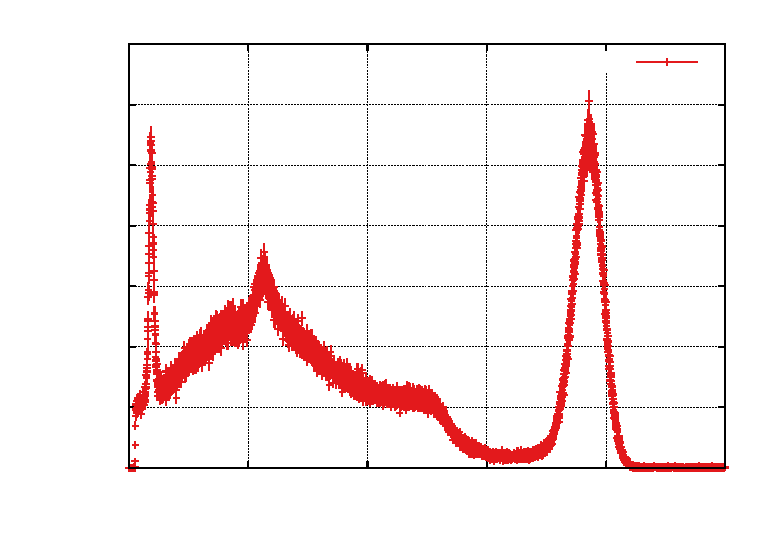
\includegraphics{./plots/szintillator/caesium}}%
    \gplfronttext
  \end{picture}%
\endgroup

	\caption{Anpassung einer Gaußfunktion an den Rückstreupeak von \isotope[137]{Cs}}
	\label{fig:fit_rueck_szinti}
\end{figure}
Die resultierenden Anpassungsparameter wurden in Tabelle \ref{tab:fit_rueck_szinti} aufgetragen.
\begin{table}[ht]
	\centering
	\begin{tabular}{lSSSSSS}
\toprule
Isotop & \multicolumn{2}{c}{Amplitude} & \multicolumn{2}{c}{Schwerpunkt} & \multicolumn{2}{c}{Standardabweichung}\\
       & {$A$} & {$\Delta A$} & {$n$} & {$\Delta n$} & {$\sigma$} & {$\Delta \sigma$}\\
\midrule
\isotope[60]{Co}        & 98.0   & 2.3         & 1374.8 & 3.6    & 145.4  & 5.0 \\
\isotope[137]{Cs}        & 179.0  & 3.0         & 1144.3 & 1.6    & 84.2   & 1.8 \\
\bottomrule
\end{tabular}
	\caption{Ergebnisse der Anpassung von Gaußfunktionen an die Rückstreupeaks. Es ist zu beachten, dass bei \co{} zwei Rückstreupeaks zu erwarten sind, diese jedoch so nah beieinander liegen, dass deren Summe ungefähr eine Gaußform aufweist. Daher wurde an diese nur eine Anpassung durchgeführt wird.}
	\label{tab:fit_rueck_szinti}
\end{table}
Zur Bestimmung des Peak-to-Total Verhältnisses der mittleren Energie der beiden Linien von \isotope[60]{Co} muss die Summe der Photopeaks im Spektrum berechnet werden.
Mit den Werten aus Tabelle \ref{tab:kalibrierungslinien_szinti} und Gleichung \eqref{eq:integral_peak} berechnet sich diese zu:
\begin{align*}
	N_\mathrm{Photo.} &= N_\mathrm{Photo.}(E_\gamma = \SI{780.580}{\kilo\electronvolt}) +  N_\mathrm{Photo.}(E_\gamma = \SI{860.086}{\kilo\electronvolt})\\
	&= (\num{116181 +- 972}) + (\num{106402 +- 771})\\
	&= \num{222582 +- 1241}
\end{align*}
Nun kann das Peak-to-Total Verhältnis $P/T$ durch:
\begin{align}
	\label{eq:ptt}
	P/T = \frac{N_\mathrm{Photo.}}{N_\mathrm{tot.} - N_\mathrm{R"uck.}}
\end{align}
berechnet werden.
Dies wurde in Tabelle \ref{tab:ptt_szinti} für die mittlere Energie der beiden Cobalt Linien und der Caesium Linie durchgeführt.
\begin{table}[ht]
	\centering
	\resizebox{\textwidth}{!}{
	\begin{tabular}{lrrrrrrSS}
\toprule
{Isotop} & {$N_\mathrm{tot.}$} & {$\Delta N_\mathrm{tot.}$} & {$N_\mathrm{Photo.}$} & {$\Delta N_\mathrm{Photo.}$} & {$N_\mathrm{R"uck.}$} & {$\Delta N_\mathrm{R"uck.}$} & {$P/T$}   & {$\Delta P/T$} \\
\midrule
\isotope[60]{Co} & 1301431    & 1219   & 222582    & 1241   & 35707         & 1464   & 17.59 \% & 0.12 \% \\
\isotope[137]{Cs} & 1319403    & 1226   & 304462    & 2279   & 37801         & 1012   & 23.76 \% & 0.18 \% \\
\bottomrule
\end{tabular}
	}
	\caption{Peak-to-Total Verhältnis $P/T$ der beiden Isotope \co{} und \cs{} für den Szintillationsdetektor. Aufgetragen ist die totale Anzahl der Ereignisse $N_\mathrm{tot.}$ (ohne Untergrund), die Anzahl der Ereignisse in den Photopeaks $N_\mathrm{Photo.}$ und die Anzahl der Ereignisse im Rückstreupeak $N_\mathrm{R"uck.}$. Die Anzahl der Ereignisse im Photopeak $N_\mathrm{Photo.}$ besteht bei \co{} aus der Summe der Ereignisse beider Photopeaks.}
	\label{tab:ptt_szinti}
\end{table}
Man sieht, dass das Peak-to-Total Verhältnis mit steigender Energie abzunehmen scheint, was dadurch zu erklären ist, dass der Wirkungsquerschnitt des Photoeffekts mit steigender Energie sinkt (vgl. Abschnitt \ref{sec:theo_photoeffekt}).

\subsubsection{Absolute Peakeffizienz}
\label{sec:absolute_peakeffizienz_szinti}
Zur Bestimmung der absoluten Peakeffizienz des Detektors wird die Aktivität der \cs{}-Quelle benötigt. Da in \cite{anleitung} die Aktivität der Quelle $A_0$ im April 1985 gegeben ist, kann mithilfe des Zerfallsgesetzes
\begin{align}
	A(t) = A_0 \exp\left( - \frac{\ln(2)\, t}{t_{1/2}} \right)
\end{align}
die Aktivität zum Zeitpunkt der Durchführung $t = \SI{30.03 +- 0.05}{a}$ berechnet werden.
Mit der gegebenen Aktivität $A_0 = \SI{25 +- 1}{\micro Ci}$ (der Fehler wurde gemäß der angegebenen signifikanten Stellen abgeschätzt) und der Halbwertszeit von \cs{} $t_{1/2} = \SI{30.17 +- 0.03}{a}$ aus \cite{nist} folgt zum Zeitpunkt der Durchführung:
\begin{align}
	\label{eq:aktivitaet_caesium}
	A = \SI{12.5 +- 0.6}{\micro Ci}
\end{align}
Mit dem Abstand der Quelle vom Detektor $d = \SI{17.8 +- 0.2}{cm}$, dem Radius des Detektors $r_\mathrm{NaI(Tl)} = \SI{24 +- 0.5}{mm}$, der Messdauer $T = \SI{720 +- 1}{\second}$ und der Anzahl der Ereignisse im Photopeak des Caesium-Spektrums aus Tabelle \ref{tab:ptt_szinti} folgt für die absolute Peakeffizienz (Gleichung \ref{eq:peakeffizienz}):
\begin{align}
	\mathcal{E}_\mathrm{NaI(Tl)} = \SI{20.1 +- 1.4}{\percent}
\end{align}
Dabei wird aufgrund der Komplexität auf Angabe einer ausführlichen Fehlerformel verzichtet.
Anschaulich bedeutet dies, dass etwa jedes fünfte Gammaquant, welches in Richtung des Detektors emittiert wird, in den Photopeak des Spektrums fällt.

\subsection{Germanium Halbleiterdetektor}
Viele der folgenden Aufgaben erfolgen in Analogie zur Auswertung für den NaI(Tl) Szintillationsdetektor, so dass hier nicht alles wiederholt werden soll.
Dies betrifft insbesondere Formeln für die Fehler.

\subsubsection{Detektorsignal des Halbleiterdetektor}
Im Folgenden soll analog zu Abschnitt \ref{sec:detektorsignal_szinti} das Detektorsignal an Vor- und Hauptverstärker des Ge-Halbleiterdetektors bestimmt werden.
Die genannten Größen und ihre Fehler werden in Analogie zum Szintillationsdetektor bestimmt.
Zunächst soll das Signal am Vorverstärker des Halbleiterdetektors in Abbildung \ref{fig:signal_ger_vor} betrachtet werden.
Die Impulsform ist nahezu identisch mit der des Szintillationsdetektors mit der Ausnahme, dass das Signal hier einen positiven Spannungsausschlag mit der Amplitude $\Delta U = \SI{0.29 +-0.01}{\volt}$ (Anstiegszeit $<\SI{1}{\micro\second}$) aufweist.
Auch der exponentielle Abfall mit der Signaldauer $\Delta t = \SI{137 +- 5}{\micro\second}$ (von 10 \% auf 10\%) ist wiederzuerkennen, wobei dieser in dem Fall nicht durch den Zerfall angeregter Zustände zu erklären ist, sondern auf die Ladungssammlung im Halbleiterkristall zurückzuführen ist.
\begin{figure}[ht]
	\centering
	\begin{subfigure}[b]{0.7\textwidth}
		\centering
		\includegraphics[width=0.7\textwidth]{./figures/signale/vor_ger_abgeschnitten.jpg}
		\caption{Am Ausgang des Vorverstärkers. Die eingestellten Skalenfaktoren am Oszilloskop betragen \SI{50}{\milli\volt\per\division} für die Vertikale und \SI{25}{\micro\second\per\division} in der Horizontalen.}
		\label{fig:signal_ger_vor}
	\end{subfigure}

	\begin{subfigure}[b]{0.7\textwidth}
		\centering
		\includegraphics[width=0.7\textwidth]{./figures/signale/haupt_ger_abgeschnitten.jpg}
		\caption{Am Ausgang des Hauptverstärkers. Die eingestellten Skalenfaktoren am Oszilloskop betragen \SI{1}{\volt\per\division} für die Vertikale und \SI{5}{\micro\second\per\division} in der Horizontalen.}
		\label{fig:signal_ger_haupt}
	\end{subfigure}
	\caption{Signalformen am Halbleiterdetektor. Die horizontalen Linien markieren \SI{0}{\volt}.}
\end{figure}
Betrachtet man nun das Signal am Hauptverstärker in Abbildung \ref{fig:signal_ger_haupt}, so beobachtet man einen gaußförmigen Impuls mit einer Signalamplitude von $\Delta U = \SI{5.1 +- 0.2}{\volt}$ und einer Signaldauer von $\Delta t = \SI{22 +- 1}{\micro\second}$.
Im Gegensatz zum Hauptverstärker des Szintillationsdetektors kann kein Überschwingen am unipolaren Ausgang des Verstärkers beobachtet werden.
Man beobachtet eine Kürzung des Signals durch den Hauptverstärker um etwa eine Größenordnung.
Der Vergleich der Impulshöhen macht auch hier wenig Sinn, da diese von unabhängigen Ereignissen stammen, dennoch sollte diese proportional zur im Halbleiter deponierten Energie sein.

\subsubsection{Aufnahme der Gammaspektren von \ch{^{60}Co}, \ch{^{137}Cs}, \ch{^{152}Eu} und des Untergrundspektrums}
Die Aufnahme der Spektren und des Untergrunds erfolgt mit dem Halbleiterdetektor analog zum Szintillationsdetektor.
Nach erfolgter Einstellung der Verstärkung (so dass das breiteste Spektrum die zur Verfügung stehenden 8192 Kanäle des Vielkanalanalysators möglichst komplett ausnutzt) werden ein Untergrund- und die drei Gammaspektren von \co{}, \cs{} und \isotope[152]{Eu} über jeweils \SI{720}{\second} aufgenommen.
Zur Bestimmung der absoluten Peakeffizienz werden in Tabelle \ref{tab:abstand_halbleiterdetektor} erneut die Abstände der Proben vom Detektor festgehalten.
\begin{table}[h]
	\centering
	\begin{tabular}{lSS}
\toprule
Isotop & {$d / \si{cm}$} & {$\Delta d / \si{cm}$} \\ \midrule
\isotope[60]{Co} & 3.0 & 0.2 \\
\isotope[137]{Cs} & 20.1 & 0.2 \\
\isotope[152]{Eu} & 22.8 & 0.2 \\ \bottomrule
\end{tabular}
	\caption{Abstände $d$ der Proben vom Halbleiterdetektor}
	\label{tab:abstand_halbleiterdetektor}
\end{table}
Das Untergrundspektrum sowie beispielhaft der Vergleich des unkorrigierten und korrigierten \cs-Spektrums sind in \ref{fig:abzug_untergrund_halb} gezeigt.
\begin{figure}[hp]
	\centering
	\begin{subfigure}[b]{0.65\textwidth}
		\resizebox{!}{0.275\textheight}{
			\input{./plots/halbleiter/untergrund.tex}
		}
		\caption{Untergrund des Ge-Halbleiterdetektors}
		\label{fig:untergrund_halb}
	\end{subfigure}
	
	\begin{subfigure}[b]{0.65\textwidth}
		\resizebox{!}{0.275\textheight}{
			\input{./plots/halbleiter/caesium_mit_untergrund.tex}
		}
		\caption{Untergrundbehaftetes \isotope[173]{Cs}-Spektrum}
		\label{fig:caesium_mit_untergrund}
	\end{subfigure}
	
	\begin{subfigure}[b]{0.65\textwidth}
		\resizebox{!}{0.275\textheight}{
			\input{./plots/halbleiter/caesium_darstellung.tex}
		}
		\caption{\isotope[137]{Cs}-Spektrum mit subtrahiertem Untergrund}
		\label{fig:caesium_ohne_untergrund}
	\end{subfigure}
	\caption{Subtraktion des gemessenen Untergrundes von dem \isotope[137]{Cs}-Spektrum. Die Spektren wurden mit einer Messdauer von $t = \SI{720}{\second}$ aufgenommen. Der Untergrund ist im Vergleich zu dem Gammaspektrum sehr klein, so dass die Korrektur praktisch nicht sichtbar ist.}
	\label{fig:abzug_untergrund_halb}
\end{figure}


\subsubsection{Energiekalibrierung}
\label{sec:kalibrierung_halb}
\begin{figure}[ht]
	\centering
	\resizebox{0.85\textwidth}{!}{
		\input{./plots/halbleiter/energiekalibrierung/caesium_darstellung.tex}
	}
	\caption{Anpassung für die Linie im Gammaspektrum von Caesium}
	\label{fig:fit_caesium}
\end{figure}
Wie beim Sztintillationsdetektor wird auch für den Halbeiterdetektor eine Energiekalibrierung durchgeführt, indem an die gefundenen Linien im Gammaspektrum der Proben eine Kurve der Form \eqref{eq:gaussfithypothese} angepasst wird.
Im Gegensatz zum NaI(Tl)-Detektor kann jedoch auch die Europiumlinie von \SI{1085.914}{\kilo\electronvolt} deutlich gesehen und zur Kalibrierung genutzt werden.
Es ergeben sich die in Tabelle \ref{tab:kalibrierungslinien_halb} festgehaltenen Werte für die Anpassungen und zugehörigen Gammaenergien aller drei Quellen.
\begin{table}[ht]
	\centering
	\resizebox{\textwidth}{!}{
	\begin{tabular}{lSSSSSSS}
	\toprule
	Isotop & {Gammaenergie} & \multicolumn{2}{c}{Amplitude} & \multicolumn{2}{c}{Schwerpunkt} & \multicolumn{2}{c}{Standardabweichung}\\
	& {$E_{\gamma}$ / \si{\kilo\electronvolt}} & {$A$} & {$\Delta A$} & {$n$} & {$\Delta n$} & {$\sigma$} & {$\Delta \sigma$}\\
	\midrule
Co & 1173.237 & 10512.8 & 241.6 & 5819.34 & 0.07 & 3.94 & 0.07 \\
Co & 1332.501 & 8750.2  & 230.6 & 6612.25 & 0.07 & 4.25 & 0.08 \\
Cs & 661.660  & 30775.2 & 394.3 & 3271.54 & 0.03 & 3.12 & 0.03 \\
Eu & 121.783  & 23990.4 & 605.3 & 583.33  & 0.05 & 2.18 & 0.05 \\
Eu & 244.699  & 4660.0  & 99.6  & 1195.92 & 0.05 & 2.35 & 0.05 \\
Eu & 344.281  & 11083.5 & 174.0 & 1691.53 & 0.04 & 2.61 & 0.03 \\
Eu & 778.903  & 2008.9  & 30.3  & 3854.90 & 0.05 & 3.24 & 0.04 \\
Eu & 964.131  & 1796.2  & 29.5  & 4777.38 & 0.05 & 3.48 & 0.05 \\
Eu & 1085.914 & 1055.9  & 18.1  & 5384.05 & 0.06 & 3.66 & 0.06 \\
Eu & 1112.116 & 1332.3  & 37.9  & 5514.44 & 0.09 & 3.78 & 0.09 \\
Eu & 1408.011 & 1534.0  & 33.5  & 6987.49 & 0.06 & 4.17 & 0.07 \\
	\bottomrule
\end{tabular}
	}
	\caption{Anpassungsergebnisse zur Energiekalibrierung für den Ge-Halbleiterdetektor}
	\label{tab:kalibrierungslinien_halb}
\end{table}
Da die Daten offensichtlich einen linearen Zusammenhang auf dem gesamten Bereich nahelegen, wird zur Anpassung eine lineare Funktion der Form $mx + b$ gewählt (analog zum NaI(Tl) Detektor).
Das Ergebnis der Anpassung ist in Abbildung \ref{fig:kalibrierung_halb} zu sehen.
\begin{figure}[ht]
	\centering
	\begin{tabular}{lSSSSSSS}
	\toprule
	Isotop & {Gammaenergie} & \multicolumn{2}{c}{Amplitude} & \multicolumn{2}{c}{Schwerpunkt} & \multicolumn{2}{c}{Standardabweichung}\\
	& {$E_{\gamma}$ / \si{\kilo\electronvolt}} & {$A$} & {$\Delta A$} & {$n$} & {$\Delta n$} & {$\sigma$} & {$\Delta \sigma$}\\
	\midrule
Co & 1173.237 & 10512.8 & 241.6 & 5819.34 & 0.07 & 3.94 & 0.07 \\
Co & 1332.501 & 8750.2  & 230.6 & 6612.25 & 0.07 & 4.25 & 0.08 \\
Cs & 661.660  & 30775.2 & 394.3 & 3271.54 & 0.03 & 3.12 & 0.03 \\
Eu & 121.783  & 23990.4 & 605.3 & 583.33  & 0.05 & 2.18 & 0.05 \\
Eu & 244.699  & 4660.0  & 99.6  & 1195.92 & 0.05 & 2.35 & 0.05 \\
Eu & 344.281  & 11083.5 & 174.0 & 1691.53 & 0.04 & 2.61 & 0.03 \\
Eu & 778.903  & 2008.9  & 30.3  & 3854.90 & 0.05 & 3.24 & 0.04 \\
Eu & 964.131  & 1796.2  & 29.5  & 4777.38 & 0.05 & 3.48 & 0.05 \\
Eu & 1085.914 & 1055.9  & 18.1  & 5384.05 & 0.06 & 3.66 & 0.06 \\
Eu & 1112.116 & 1332.3  & 37.9  & 5514.44 & 0.09 & 3.78 & 0.09 \\
Eu & 1408.011 & 1534.0  & 33.5  & 6987.49 & 0.06 & 4.17 & 0.07 \\
	\bottomrule
\end{tabular}
	\caption{Energiekalibrierung des Ge-Halbleiterdetektors. Die Fehler sind zu klein, um gesehen werden zu können.}
	\label{fig:kalibrierung_halb}
\end{figure}  
Die Anpassungsergebnisse durch \texttt{gnuplot} lauten:
\begin{align}
	m &= \SI{0.200839 +- 0.000010}{\kilo\electronvolt} \nonumber\\
	b &= \SI{4.589 +- 0.046}{\kilo\electronvolt}
	\label{eq:kalibrierung_halb}
\end{align}


\subsubsection{Bestimmung der Halbwertsbreite}
\label{sec:fwhm_halb}
Zur Bestimmung der Halbwertsbreiten für den Halbleiterdetektor kann erneut die Anpassung der Gaußfunktionen an die jeweiligen Linien verwendet werden, welche bereits bei der Energiekalibrierung in Abschnitt \ref{sec:kalibrierung_halb} durchgeführt wurden.
Analog zum Szintillationsdetektor wird dabei die volle Halbwertsbreite (FWHM) aus der Standardabweichung $\sigma$ der Anpassung berechnet.
Mit den Anpassungsergebnissen aus Tabelle \ref{tab:kalibrierungslinien_halb} kann dementsprechend die Halbwertsbreite in Einheiten der Kanalnummer berechnet werden.
Diese kann mithilfe der Energiekalibrierung in Abschnitt \ref{sec:kalibrierung_halb} in Einheiten der Energie umgerechnet werden, indem die Halbwertsbreite in Einheiten der Kanalnummer mit der Steigung der Kalibrierungsgeraden multipliziert wird.
Die berechneten Breiten wurden in Tabelle \ref{tab:fwhm_halb} zusammengetragen.
\begin{table}[ht]
	\centering
	\begin{tabular}{lSSSSS}
\toprule
Isotop & {Gammaenergie} & {FWHM} & {$\Delta \text{FWHM}$} & {FWHM} & {$\Delta \text{FWHM}$}\\
       & {$E_\gamma$ / \si{keV}}             & \multicolumn{2}{c}{Kanäle} & \multicolumn{2}{c}{\si{keV}} \\
\midrule
Co & 1173.237 & 9.28  & 0.16 & 1.864 & 0.031 \\
Co & 1332.501 & 10.00 & 0.19 & 2.008 & 0.037 \\
Cs & 661.660  & 7.34  & 0.07 & 1.475 & 0.013 \\
Eu & 121.783  & 5.12  & 0.10 & 1.029 & 0.020 \\
Eu & 244.699  & 5.54  & 0.11 & 1.113 & 0.021 \\
Eu & 344.281  & 6.14  & 0.07 & 1.232 & 0.014 \\
Eu & 778.903  & 7.63  & 0.10 & 1.533 & 0.019 \\
Eu & 964.131  & 8.19  & 0.11 & 1.645 & 0.021 \\
Eu & 1085.914 & 8.62  & 0.13 & 1.731 & 0.026 \\
Eu & 1112.116 & 8.90  & 0.20 & 1.787 & 0.039 \\
Eu & 1408.011 & 9.82  & 0.15 & 1.972 & 0.031 \\
\bottomrule
\end{tabular}
	\caption{Volle Halbwertsbreiten der zur Kalibration verwendeten Linien in den Spektren von \isotope[60]{Co}, \isotope[137]{Cs} und \isotope[152]{Eu}.}
	\label{tab:fwhm_halb}
\end{table}
Im Gegensatz zum Szintillationsdetektor sieht man in diesem Fall einen eindeutigen Anstieg der Halbwertsbreiten mit steigender Gammaenergie.
Dies ist in erster Linie auf die wesentlich bessere Energiekalibrierung des Halbleiterdetektors zurückzuführen.\\
\\
Schließlich soll der Einfluss von intrinsischer Detektor-Halbwertsbreite $\Delta E_\mathrm{d}$, welche auf dem statistischen Prozess der Ladungssammlung im Ge-Kristall basiert \cite{anleitung} und der elektronische Teil der Halbwertsbreite $\Delta E_\mathrm{e}$, welche von der verwendeten Verstärkerelektronik abhängt, untersucht werden.
Die mit dem Vielkanalysator beobachtete Linienbreite $\Delta E$ setzt sich aus beiden Anteilen zusammen und wird beschrieben durch \cite{anleitung}:
\begin{align}
	\Delta E(E_\gamma) = \sqrt{(\Delta E_\mathrm{d}(E_\gamma))^2 + (\Delta E_\mathrm{e})^2}
\end{align}
Darüber hinaus ist die intrinsische Detektor-Energiebreite abhängig von der Gammaenergie $E_\gamma$ und gegeben durch:
\begin{align}
	\label{eq:prop_energiebreite}
	\Delta E_\mathrm{d}(E_\gamma) \propto \sqrt{E_\gamma}
\end{align}
Mithilfe dieser Überlegungen ist es möglich die intrinsische Halbwertsbreite sowie den elektronischen Teil mit den Anpassungen aus Tabelle \ref{tab:fwhm_halb} zu bestimmen.
Dazu betrachtet man das Quadrat der beobachteten Breite unter Beachtung der Abhängigkeit aus Gleichung \eqref{eq:prop_energiebreite}:
\begin{align}
	\Delta E^2 = (\Delta E_\mathrm{d})^2 + (\Delta E_\mathrm{e})^2 = \lambda^2 \cdot E_\gamma + (\Delta E_\mathrm{e})^2
\end{align}
Liniearisiert man diesen Zusammenhang indem man die quadrierte beobachtete Halbwertsbreite $\Delta E^2$ gegen die Gammaenergie $E_\gamma$ aufträgt, so kann man die Abhängigkeit der intrinsischen Breite des Detektors von der Gammaenergie aus der Steigung der Geraden extrahieren und den elektronischen Teil aus deren Achsenabschnitt.
Die Linearisierung wurde in Abbildung \ref{fig:lin_fwhm} dargestellt.
\begin{figure}[ht]
	\centering
	\input{./plots/halbleiter/linearisierung_halbwertsbreiten.tex}
	\caption{Linearisierung zur Bestimmung der intrinsischen und elektronischen Anteile des verwendeten Ge-Halbleiterdetektors.}
	\label{fig:lin_fwhm}
\end{figure}
Die Anpassung der Geraden liefert die Parameter:
\begin{align*}
	\lambda^2 &= \SI{2.15 +- 0.08e-3}{\kilo\electronvolt}\\
	(\Delta E_\mathrm{e})^2 &= \SI{0.75 +- 0.05}{\kilo\electronvolt\squared}
\end{align*}
Zunächst soll die Proportionalität der intrinsischen Halbwertsbreite bestimmt werden.
Dazu reicht es, $\lambda$ zu bestimmen\footnote{
Fehlerfortpflanzung bei Bildung der Quadratwurzel: $\Delta (\sqrt{x}) = \frac{\Delta x}{2 \sqrt{x}} $
}:
\begin{align*}
	\lambda = \SI{4.64 +-0.08e-2}{\kilo\electronvolt\tothe{\frac{1}{2}}}
\end{align*}
Dann ist der Zusammenhang der intrinsischen Halbwertsbreite gegeben durch:
\begin{align}
	\Delta E_\mathrm{d} = \SI{4.64 +-0.08e-2}{\kilo\electronvolt\tothe{\frac{1}{2}}} \cdot \sqrt{E_\gamma}
\end{align}
Schließlich kann der elektronische Anteil bestimmt werden, was ebenfalls durch Bildung der Quadratwurzel geschieht:
\begin{align}
	\Delta E_\mathrm{e} = \SI{0.87 +- 0.03}{\kilo\electronvolt}
\end{align}
Betrachtet man beide Anteile an der Halbwertsbreite, so sieht man, dass der elektronische Anteil die Breite bis ca. \SI{350}{\kilo\electronvolt} dominiert.
Für größere Gammaenergien beginnt die intrinsische Breite des Detektors die beobachtete Breite zu dominieren.


\subsubsection{Peak-to-Total-Verhältnis}
Analog zum Abschnitt \ref{sec:ptt_szinti} soll das Peak-to-Total-Verhältnis berechnet werden.
Dazu berechnet man durch Integration über die an den Peaks angepassten Gaußfunktionen die Gesamtzahl der in den Peak gefallenen Quanten.
Mit den Anpassungen an die Photopeaks aus Abschnitt \ref{sec:kalibrierung_halb} kann direkt die Anzahl der Ereignisse berechnet werden.
Darüber hinaus muss noch eine Anpassung an die Rückstreupeaks erfolgen, welche hier exemplarisch am Rückstreupeak von \cs{} in Abbildung \ref{fig:rueck_halb_cs} dargestellt werden soll.
\begin{figure}[ht]
	\centering
	% GNUPLOT: LaTeX picture with Postscript
\begingroup
  \makeatletter
  \providecommand\color[2][]{%
    \GenericError{(gnuplot) \space\space\space\@spaces}{%
      Package color not loaded in conjunction with
      terminal option `colourtext'%
    }{See the gnuplot documentation for explanation.%
    }{Either use 'blacktext' in gnuplot or load the package
      color.sty in LaTeX.}%
    \renewcommand\color[2][]{}%
  }%
  \providecommand\includegraphics[2][]{%
    \GenericError{(gnuplot) \space\space\space\@spaces}{%
      Package graphicx or graphics not loaded%
    }{See the gnuplot documentation for explanation.%
    }{The gnuplot epslatex terminal needs graphicx.sty or graphics.sty.}%
    \renewcommand\includegraphics[2][]{}%
  }%
  \providecommand\rotatebox[2]{#2}%
  \@ifundefined{ifGPcolor}{%
    \newif\ifGPcolor
    \GPcolortrue
  }{}%
  \@ifundefined{ifGPblacktext}{%
    \newif\ifGPblacktext
    \GPblacktexttrue
  }{}%
  % define a \g@addto@macro without @ in the name:
  \let\gplgaddtomacro\g@addto@macro
  % define empty templates for all commands taking text:
  \gdef\gplbacktext{}%
  \gdef\gplfronttext{}%
  \makeatother
  \ifGPblacktext
    % no textcolor at all
    \def\colorrgb#1{}%
    \def\colorgray#1{}%
  \else
    % gray or color?
    \ifGPcolor
      \def\colorrgb#1{\color[rgb]{#1}}%
      \def\colorgray#1{\color[gray]{#1}}%
      \expandafter\def\csname LTw\endcsname{\color{white}}%
      \expandafter\def\csname LTb\endcsname{\color{black}}%
      \expandafter\def\csname LTa\endcsname{\color{black}}%
      \expandafter\def\csname LT0\endcsname{\color[rgb]{1,0,0}}%
      \expandafter\def\csname LT1\endcsname{\color[rgb]{0,1,0}}%
      \expandafter\def\csname LT2\endcsname{\color[rgb]{0,0,1}}%
      \expandafter\def\csname LT3\endcsname{\color[rgb]{1,0,1}}%
      \expandafter\def\csname LT4\endcsname{\color[rgb]{0,1,1}}%
      \expandafter\def\csname LT5\endcsname{\color[rgb]{1,1,0}}%
      \expandafter\def\csname LT6\endcsname{\color[rgb]{0,0,0}}%
      \expandafter\def\csname LT7\endcsname{\color[rgb]{1,0.3,0}}%
      \expandafter\def\csname LT8\endcsname{\color[rgb]{0.5,0.5,0.5}}%
    \else
      % gray
      \def\colorrgb#1{\color{black}}%
      \def\colorgray#1{\color[gray]{#1}}%
      \expandafter\def\csname LTw\endcsname{\color{white}}%
      \expandafter\def\csname LTb\endcsname{\color{black}}%
      \expandafter\def\csname LTa\endcsname{\color{black}}%
      \expandafter\def\csname LT0\endcsname{\color{black}}%
      \expandafter\def\csname LT1\endcsname{\color{black}}%
      \expandafter\def\csname LT2\endcsname{\color{black}}%
      \expandafter\def\csname LT3\endcsname{\color{black}}%
      \expandafter\def\csname LT4\endcsname{\color{black}}%
      \expandafter\def\csname LT5\endcsname{\color{black}}%
      \expandafter\def\csname LT6\endcsname{\color{black}}%
      \expandafter\def\csname LT7\endcsname{\color{black}}%
      \expandafter\def\csname LT8\endcsname{\color{black}}%
    \fi
  \fi
    \setlength{\unitlength}{0.0500bp}%
    \ifx\gptboxheight\undefined%
      \newlength{\gptboxheight}%
      \newlength{\gptboxwidth}%
      \newsavebox{\gptboxtext}%
    \fi%
    \setlength{\fboxrule}{0.5pt}%
    \setlength{\fboxsep}{1pt}%
\begin{picture}(7200.00,5040.00)%
    \gplgaddtomacro\gplbacktext{%
      \csname LTb\endcsname%
      \put(946,704){\makebox(0,0)[r]{\strut{}$0$}}%
      \put(946,1286){\makebox(0,0)[r]{\strut{}$200$}}%
      \put(946,1867){\makebox(0,0)[r]{\strut{}$400$}}%
      \put(946,2449){\makebox(0,0)[r]{\strut{}$600$}}%
      \put(946,3030){\makebox(0,0)[r]{\strut{}$800$}}%
      \put(946,3612){\makebox(0,0)[r]{\strut{}$1000$}}%
      \put(946,4193){\makebox(0,0)[r]{\strut{}$1200$}}%
      \put(946,4775){\makebox(0,0)[r]{\strut{}$1400$}}%
      \put(1078,484){\makebox(0,0){\strut{}$0$}}%
      \put(2223,484){\makebox(0,0){\strut{}$1000$}}%
      \put(3368,484){\makebox(0,0){\strut{}$2000$}}%
      \put(4513,484){\makebox(0,0){\strut{}$3000$}}%
      \put(5658,484){\makebox(0,0){\strut{}$4000$}}%
      \put(6803,484){\makebox(0,0){\strut{}$5000$}}%
      \put(1467,3030){\rotatebox{-270}{\makebox(0,0)[l]{\strut{}Röntgenlinie}}}%
      \put(2371,2914){\rotatebox{-270}{\makebox(0,0)[l]{\strut{}Rückstreupeak}}}%
      \put(4009,1635){\rotatebox{-270}{\makebox(0,0)[l]{\strut{}Compton-Kante}}}%
      \put(5807,3030){\rotatebox{-270}{\makebox(0,0)[l]{\strut{}\SI{661.660}{keV}}}}%
    }%
    \gplgaddtomacro\gplfronttext{%
      \csname LTb\endcsname%
      \put(176,2739){\rotatebox{-270}{\makebox(0,0){\strut{}Ereignisse $N$}}}%
      \put(3940,154){\makebox(0,0){\strut{}Kanal $n$}}%
    }%
    \gplbacktext
    \put(0,0){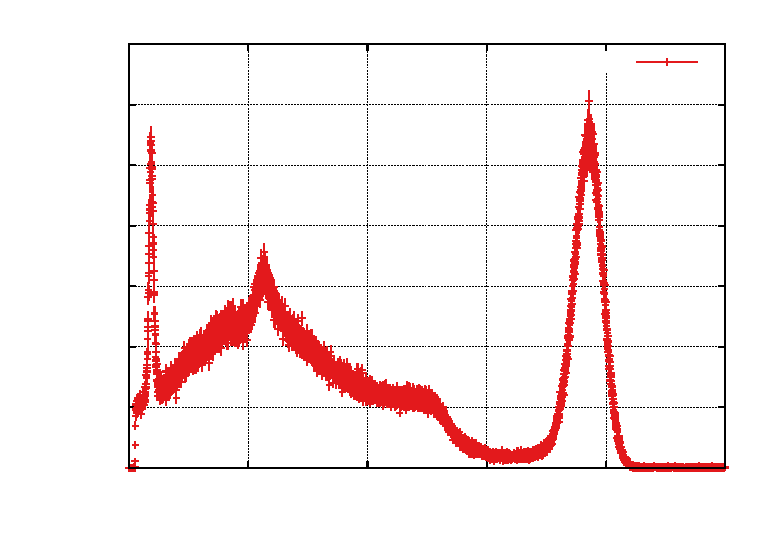
\includegraphics{./plots/szintillator/caesium}}%
    \gplfronttext
  \end{picture}%
\endgroup

	\caption{Anpassung einer Gaußfunktion an den Rückstreupeak von \cs{}}
	\label{fig:rueck_halb_cs}
\end{figure}
Die Anpassungsparameter wurden in Tabelle \ref{tab:fit_rueck_halb} zusammengefasst.
\begin{table}[ht]
	\centering
	\begin{tabular}{lSSSSSS}
\toprule
Isotop & \multicolumn{2}{c}{Amplitude} & \multicolumn{2}{c}{Schwerpunkt} & \multicolumn{2}{c}{Standardabweichung}\\
       & {$A$} & {$\Delta A$} & {$n$} & {$\Delta n$} & {$\sigma$} & {$\Delta \sigma$}\\
\midrule
\isotope[60]{Co}        & 65.0   & 2.9         & 1118.5 & 3.0    & 75.9  & 4.8 \\
\isotope[137]{Cs}        & 193.6  & 6.1         & 920.0 & 1.1    & 30.2   & 1.2 \\
\bottomrule
\end{tabular}
	\caption{Ergebnisse der Anpassung von Gaußfunktionen an die Rückstreupeaks}
	\label{tab:fit_rueck_halb}
\end{table}
Berechnet man nun durch Integration die Anzahl der Ereignisse in den verschiedenen Peaks so erhält man Tabelle \ref{tab:ptt_halb}, wobei das Peak-to-Total Verhältnis durch Gleichung \eqref{eq:ptt} berechnet wurde.
\begin{table}[ht]
	\centering
	\resizebox{\textwidth}{!}{
		\begin{tabular}{lrrrrrrSS}
	\toprule
	{Isotop} & {$N_\mathrm{tot.}$} & {$\Delta N_\mathrm{tot.}$} & {$N_\mathrm{Photo.}$} & {$\Delta N_\mathrm{Photo.}$} & {$N_\mathrm{R"uck.}$} & {$\Delta N_\mathrm{R"uck.}$} & {$P/T$}   & {$\Delta P/T$} \\
	\midrule
	\isotope[60]{Co} & 1370053    & 1261   & 196984    & 4184   & 12367         & 950  & 14.51 \% & 0.31 \% \\
	\isotope[137]{Cs} & 1344655    & 1250   & 240566    & 3731   & 14660         & 740   & 18.09 \% & 0.29 \% \\
	\bottomrule
\end{tabular}
	}
	\caption{Peak-to-Total Verhältnis $P/T$ der beiden Isotope \co{} und \cs{} für den Ge-Halbleiterdetektor. Aufgetragen ist die totale Anzahl der Ereignisse $N_\mathrm{tot.}$ (ohne Untergrund), die Anzahl der Ereignisse in den Photopeaks $N_\mathrm{Photo.}$ und die Anzahl der Ereignisse im Rückstreupeak $N_\mathrm{R"uck.}$. Die Anzahl der Ereignisse im Photopeak $N_\mathrm{Photo.}$ besteht bei \co{} aus der Summe der Ereignisse beider Photopeaks.}
	\label{tab:ptt_halb}
\end{table}
Man sieht erneut die Abnahme des Peak-to-Total Verhältnisses mit steigender Energie, was in der Abnahme des Wirkungsquerschnitts mit Zunahme der Energie begründet liegt.
Außerdem stellt man fest, dass das Verhältnis kleiner ist als das des Szintillationsdetektors.


\subsubsection{Absolute Peakeffizienz}
In Abschnitt \ref{sec:absolute_peakeffizienz_szinti} wurde die Aktivität der verwendeten \cs{}-Quelle zu
\begin{align}
	A = \SI{12.5 +- 0.6}{\micro Ci}
\end{align}
bestimmt.
Nun befindet sich die Quelle im Abstand von $d = \SI{20.1 +- 0.2}{\centi\metre}$ vom Ge-Halbleiterdetektor mit dem Kristallradius $r = \SI{27.85 +- 0.05}{\milli\metre}$ entfernt.
Die Messzeit betrug auch hier $T = \SI{720 +- 1}{\second}$ und die Anzahl der Ereignisse im Photopeak lässt sich aus Tabelle \ref{tab:ptt_halb} ablesen.
Mit Gleichung \eqref{eq:peakeffizienz} folgt:
\begin{align}
	\mathcal{E}_\mathrm{Ge} = \SI{15.05 +- 0.82}{\percent}
\end{align}
Dies bedeutet, dass etwa $\SI{15}{\percent}$ der auf den Ge-Kristall einfallenden Quanten im Photopeak detektiert werden.
Der Vergleich mit Abschnitt \ref{sec:absolute_peakeffizienz_szinti} zeigt, dass der Szintillationsdetektor eine höhere Peakeffizienz bei der Energie der \cs{}-Linie aufweist.

\subsubsection{Relative Effizienz als Funktion der Gammaenergie}
Zur Bestimmung der relativen Effizienz des Detektors über den vermessenen Energiebereich können die in \cite{anleitung} aufgelisteten relativen Intensitäten der \eu{}-Linien genutzt werden, welche im Folgenden mit $I_\mathrm{0}$ bezeichnet werden.
Um die Intensität $I$ der einzelnen Linien experimentell zu bestimmen, berechnen wir erneut die Anzahl der Ereignisse $N$ im Peak der Linie durch Integration über die in Tabelle \ref{tab:kalibrierungslinien_halb} angepasste Gaußfunktionen.
Um die Anzahl der Ereignisse $N$ in eine relative Intensität $I$ umzurechnen, wird eine Linie zur Normierung genutzt.
Konkret wird dazu die \SI{1408.011}{keV}-Linie von \eu{} genutzt, welche die relative Intensität \num{1000} habe.
Die Normierung erfolgt durch:
\begin{align}
	I = 1000 \cdot \frac{N}{N_\mathrm{Ref}} \qquad \Delta I = 1000 \cdot \sqrt{\frac{\Delta N^2}{N_\mathrm{Ref}^2} + \frac{N^2 \cdot \Delta N_\mathrm{Ref}^2}{N_\mathrm{Ref}^4}}
\end{align}
wobei $N_\mathrm{ref} = \num{16036 +- 428}$ die Ereigniszahl in der Referenzlinie ist. 
Anschließend führt der Vergleich der mit dem Detektor gemessenen relativen Intensität $I$ und den in \cite{anleitung} angegeben theoretischen Werten $I_0$ zu der relativen Effizienz:
\begin{align}
	\eta = \frac{I}{I_0} \qquad \Delta \eta = \frac{\Delta I}{I_0}
\end{align}
In Tabelle \ref{tab:rel_effizienz_halb} wurden die hier erwähnten Größen zusammengefasst.
\begin{table}[ht]
	\centering
	\resizebox{\textwidth}{!}{
	\begin{tabular}{SSSSSSSS}
\toprule
{$E_\gamma / \si{keV}$}  & {$N$} & {$\Delta N$} & {$I$} & {$\Delta I$} & {$I_0$} & {$\eta$} & {$\Delta \eta$} \\
\midrule
121.783 & 130801 & 4095   & 8157           & 336    & 1362.0   & 5.99      & 0.25   \\
244.699 & 27480  & 771    & 1714           & 67     & 359.0    & 4.77      & 0.19   \\
344.281  & 72396  & 1393   & 4515           & 149    & 1275.0   & 3.54      & 0.12   \\
778.903  & 16320  & 314    & 1018           & 34     & 621.6    & 1.64      & 0.06   \\
964.131  & 15663  & 326    & 977            & 33     & 693.4    & 1.41      & 0.05   \\
1085.914 & 9688   & 219    & 604            & 22     & 475.0    & 1.27      & 0.05   \\
1112.116 & 12618  & 451    & 787            & 36     & 649.0    & 1.21      & 0.06   \\
1408.011 & 16036  & 428    & 1000           &      & 1000.0   & 1.00      &       \\ \bottomrule
\end{tabular}
	}
	\caption{Normierung der Intensitäten $I$ auf die \SI{1408.011}{keV}-Linie von Europium und Berechnung der relativen Effizienz $\eta$}
	\label{tab:rel_effizienz_halb}
\end{table}
Man erkennt, wie die relative Effizienz des Detektors mit steigender Energie sinkt.
Auch dies liegt wieder in der Abnahme des Wirkungsquerschnitts für den Photoeffekt mit steigender Energie begründet.
Trägt man die relative Effizienz $\eta$ gegen die Gammaenergie $E_\gamma$ auf so erhält man Abbildung \ref{fig:effizienz_halb}.
\begin{figure}[ht]
	\centering
	\input{./plots/halbleiter/effizienz.tex}
	\caption{Relative Effizienz des Ge-Halbleiterdetektors bei verschiedenen Energien $E_\gamma$ mit Anpassung einer Exponentialfunktion}
	\label{fig:effizienz_halb}
\end{figure}
Auf dem Messbereich wird die relative Effizienz gut durch eine Exponentialfunktion:
\begin{align*}
	\eta(E_\gamma) &= A \cdot \mathrm{e}^{-\frac{E_\gamma}{B}}  + C \\
	A &= \num{7.21+-0.37} \\
	B &= \SI{364 +- 20}{keV} \\
	C &= \num{0.852 +- 0.032}
\end{align*}
beschrieben.

\subsection{Nachweis der Radioakivität in einer Probe}

Zum Ende des Versuchs wurde mit dem Halbleiterdetektor das Spektrum einer mitgebrachten Bodenprobe aufgenommen.
Die Messung erfolgte dazu in einer Bleiabschirmung über ca. \SI{16}{\hour}. Anschließend wurde ein Untergrundspektrum über eine andere Zeit (ca. \SI{24}{\hour}) aufgenommen.
Um das Spektrum vom Untergrund zu bereinigen mussten die Ereignisse anhand der Aufnahmezeit der Bodenprobe skaliert werden.
Das aufgenommene Spektrum der Bodenprobe, sowie der Untergrund und das bereinigte Spektrum, was im Folgenden weiter betrachtet wird, sind in Abbildung \ref{fig:langzeitmessung_untergrundabzug} dargestellt.
\begin{figure}[hp]
	\centering
	\begin{subfigure}[b]{0.65\textwidth}
		\resizebox{!}{0.275\textheight}{
			\input{./plots/langzeitmessung/untergrund.tex}
		}
		\caption{Untergrund des Ge-Halbleiterdetektors}
		\label{fig:untergrund}
	\end{subfigure}
	
	\begin{subfigure}[b]{0.65\textwidth}
		\resizebox{!}{0.275\textheight}{
			\input{./plots/langzeitmessung/spektrum_mit_untergrund.tex}
		}
		\caption{Untergrundbehaftetes Spektrum der Bodenprobe}
		\label{fig:probe_mit_untergrund}
	\end{subfigure}
	
	\begin{subfigure}[b]{0.65\textwidth}
		\resizebox{!}{0.28\textheight}{
			% GNUPLOT: LaTeX picture with Postscript
\begingroup
  \makeatletter
  \providecommand\color[2][]{%
    \GenericError{(gnuplot) \space\space\space\@spaces}{%
      Package color not loaded in conjunction with
      terminal option `colourtext'%
    }{See the gnuplot documentation for explanation.%
    }{Either use 'blacktext' in gnuplot or load the package
      color.sty in LaTeX.}%
    \renewcommand\color[2][]{}%
  }%
  \providecommand\includegraphics[2][]{%
    \GenericError{(gnuplot) \space\space\space\@spaces}{%
      Package graphicx or graphics not loaded%
    }{See the gnuplot documentation for explanation.%
    }{The gnuplot epslatex terminal needs graphicx.sty or graphics.sty.}%
    \renewcommand\includegraphics[2][]{}%
  }%
  \providecommand\rotatebox[2]{#2}%
  \@ifundefined{ifGPcolor}{%
    \newif\ifGPcolor
    \GPcolortrue
  }{}%
  \@ifundefined{ifGPblacktext}{%
    \newif\ifGPblacktext
    \GPblacktexttrue
  }{}%
  % define a \g@addto@macro without @ in the name:
  \let\gplgaddtomacro\g@addto@macro
  % define empty templates for all commands taking text:
  \gdef\gplbacktext{}%
  \gdef\gplfronttext{}%
  \makeatother
  \ifGPblacktext
    % no textcolor at all
    \def\colorrgb#1{}%
    \def\colorgray#1{}%
  \else
    % gray or color?
    \ifGPcolor
      \def\colorrgb#1{\color[rgb]{#1}}%
      \def\colorgray#1{\color[gray]{#1}}%
      \expandafter\def\csname LTw\endcsname{\color{white}}%
      \expandafter\def\csname LTb\endcsname{\color{black}}%
      \expandafter\def\csname LTa\endcsname{\color{black}}%
      \expandafter\def\csname LT0\endcsname{\color[rgb]{1,0,0}}%
      \expandafter\def\csname LT1\endcsname{\color[rgb]{0,1,0}}%
      \expandafter\def\csname LT2\endcsname{\color[rgb]{0,0,1}}%
      \expandafter\def\csname LT3\endcsname{\color[rgb]{1,0,1}}%
      \expandafter\def\csname LT4\endcsname{\color[rgb]{0,1,1}}%
      \expandafter\def\csname LT5\endcsname{\color[rgb]{1,1,0}}%
      \expandafter\def\csname LT6\endcsname{\color[rgb]{0,0,0}}%
      \expandafter\def\csname LT7\endcsname{\color[rgb]{1,0.3,0}}%
      \expandafter\def\csname LT8\endcsname{\color[rgb]{0.5,0.5,0.5}}%
    \else
      % gray
      \def\colorrgb#1{\color{black}}%
      \def\colorgray#1{\color[gray]{#1}}%
      \expandafter\def\csname LTw\endcsname{\color{white}}%
      \expandafter\def\csname LTb\endcsname{\color{black}}%
      \expandafter\def\csname LTa\endcsname{\color{black}}%
      \expandafter\def\csname LT0\endcsname{\color{black}}%
      \expandafter\def\csname LT1\endcsname{\color{black}}%
      \expandafter\def\csname LT2\endcsname{\color{black}}%
      \expandafter\def\csname LT3\endcsname{\color{black}}%
      \expandafter\def\csname LT4\endcsname{\color{black}}%
      \expandafter\def\csname LT5\endcsname{\color{black}}%
      \expandafter\def\csname LT6\endcsname{\color{black}}%
      \expandafter\def\csname LT7\endcsname{\color{black}}%
      \expandafter\def\csname LT8\endcsname{\color{black}}%
    \fi
  \fi
    \setlength{\unitlength}{0.0500bp}%
    \ifx\gptboxheight\undefined%
      \newlength{\gptboxheight}%
      \newlength{\gptboxwidth}%
      \newsavebox{\gptboxtext}%
    \fi%
    \setlength{\fboxrule}{0.5pt}%
    \setlength{\fboxsep}{1pt}%
\begin{picture}(7200.00,5040.00)%
    \gplgaddtomacro\gplbacktext{%
      \csname LTb\endcsname%
      \put(946,704){\makebox(0,0)[r]{\strut{}$0$}}%
      \csname LTb\endcsname%
      \put(946,1072){\makebox(0,0)[r]{\strut{}$100$}}%
      \csname LTb\endcsname%
      \put(946,1439){\makebox(0,0)[r]{\strut{}$200$}}%
      \csname LTb\endcsname%
      \put(946,1807){\makebox(0,0)[r]{\strut{}$300$}}%
      \csname LTb\endcsname%
      \put(946,2174){\makebox(0,0)[r]{\strut{}$400$}}%
      \csname LTb\endcsname%
      \put(946,2542){\makebox(0,0)[r]{\strut{}$500$}}%
      \csname LTb\endcsname%
      \put(946,2909){\makebox(0,0)[r]{\strut{}$600$}}%
      \csname LTb\endcsname%
      \put(946,3277){\makebox(0,0)[r]{\strut{}$700$}}%
      \csname LTb\endcsname%
      \put(946,3644){\makebox(0,0)[r]{\strut{}$800$}}%
      \csname LTb\endcsname%
      \put(946,4012){\makebox(0,0)[r]{\strut{}$900$}}%
      \csname LTb\endcsname%
      \put(946,4379){\makebox(0,0)[r]{\strut{}$1000$}}%
      \csname LTb\endcsname%
      \put(1555,484){\makebox(0,0){\strut{}$344$}}%
      \csname LTb\endcsname%
      \put(2509,484){\makebox(0,0){\strut{}$346$}}%
      \csname LTb\endcsname%
      \put(3463,484){\makebox(0,0){\strut{}$348$}}%
      \csname LTb\endcsname%
      \put(4418,484){\makebox(0,0){\strut{}$350$}}%
      \csname LTb\endcsname%
      \put(5372,484){\makebox(0,0){\strut{}$352$}}%
      \csname LTb\endcsname%
      \put(6326,484){\makebox(0,0){\strut{}$354$}}%
      \csname LTb\endcsname%
      \put(2032,4599){\makebox(0,0){\strut{}$69$}}%
      \csname LTb\endcsname%
      \put(3225,4599){\makebox(0,0){\strut{}$69{,}5$}}%
      \csname LTb\endcsname%
      \put(4418,4599){\makebox(0,0){\strut{}$70$}}%
      \csname LTb\endcsname%
      \put(5610,4599){\makebox(0,0){\strut{}$70{,}5$}}%
      \csname LTb\endcsname%
      \put(6803,4599){\makebox(0,0){\strut{}$71$}}%
    }%
    \gplgaddtomacro\gplfronttext{%
      \csname LTb\endcsname%
      \put(176,2541){\rotatebox{-270}{\makebox(0,0){\strut{}Ereignisse $N$}}}%
      \put(3940,154){\makebox(0,0){\strut{}Kanal $n$}}%
      \put(3940,4928){\makebox(0,0){\strut{}Energie / \si{\kilo\electronvolt}}}%
      \csname LTb\endcsname%
      \put(5816,4206){\makebox(0,0)[r]{\strut{}Messwerte}}%
    }%
    \gplgaddtomacro\gplbacktext{%
      \csname LTb\endcsname%
      \put(946,704){\makebox(0,0)[r]{\strut{}$0$}}%
      \csname LTb\endcsname%
      \put(946,1072){\makebox(0,0)[r]{\strut{}$100$}}%
      \csname LTb\endcsname%
      \put(946,1439){\makebox(0,0)[r]{\strut{}$200$}}%
      \csname LTb\endcsname%
      \put(946,1807){\makebox(0,0)[r]{\strut{}$300$}}%
      \csname LTb\endcsname%
      \put(946,2174){\makebox(0,0)[r]{\strut{}$400$}}%
      \csname LTb\endcsname%
      \put(946,2542){\makebox(0,0)[r]{\strut{}$500$}}%
      \csname LTb\endcsname%
      \put(946,2909){\makebox(0,0)[r]{\strut{}$600$}}%
      \csname LTb\endcsname%
      \put(946,3277){\makebox(0,0)[r]{\strut{}$700$}}%
      \csname LTb\endcsname%
      \put(946,3644){\makebox(0,0)[r]{\strut{}$800$}}%
      \csname LTb\endcsname%
      \put(946,4012){\makebox(0,0)[r]{\strut{}$900$}}%
      \csname LTb\endcsname%
      \put(946,4379){\makebox(0,0)[r]{\strut{}$1000$}}%
      \csname LTb\endcsname%
      \put(1555,484){\makebox(0,0){\strut{}$344$}}%
      \csname LTb\endcsname%
      \put(2509,484){\makebox(0,0){\strut{}$346$}}%
      \csname LTb\endcsname%
      \put(3463,484){\makebox(0,0){\strut{}$348$}}%
      \csname LTb\endcsname%
      \put(4418,484){\makebox(0,0){\strut{}$350$}}%
      \csname LTb\endcsname%
      \put(5372,484){\makebox(0,0){\strut{}$352$}}%
      \csname LTb\endcsname%
      \put(6326,484){\makebox(0,0){\strut{}$354$}}%
      \csname LTb\endcsname%
      \put(2032,4599){\makebox(0,0){\strut{}$69$}}%
      \csname LTb\endcsname%
      \put(3225,4599){\makebox(0,0){\strut{}$69{,}5$}}%
      \csname LTb\endcsname%
      \put(4418,4599){\makebox(0,0){\strut{}$70$}}%
      \csname LTb\endcsname%
      \put(5610,4599){\makebox(0,0){\strut{}$70{,}5$}}%
      \csname LTb\endcsname%
      \put(6803,4599){\makebox(0,0){\strut{}$71$}}%
    }%
    \gplgaddtomacro\gplfronttext{%
      \csname LTb\endcsname%
      \put(176,2541){\rotatebox{-270}{\makebox(0,0){\strut{}Ereignisse $N$}}}%
      \put(3940,154){\makebox(0,0){\strut{}Kanal $n$}}%
      \put(3940,4928){\makebox(0,0){\strut{}Energie / \si{\kilo\electronvolt}}}%
      \csname LTb\endcsname%
      \put(5816,4206){\makebox(0,0)[r]{\strut{}Messwerte}}%
      \csname LTb\endcsname%
      \put(5816,3986){\makebox(0,0)[r]{\strut{}$\Sigma$}}%
      \csname LTb\endcsname%
      \put(5816,3766){\makebox(0,0)[r]{\strut{}$\mathcal{G}_1$}}%
      \csname LTb\endcsname%
      \put(5816,3546){\makebox(0,0)[r]{\strut{}$d$}}%
    }%
    \gplbacktext
    \put(0,0){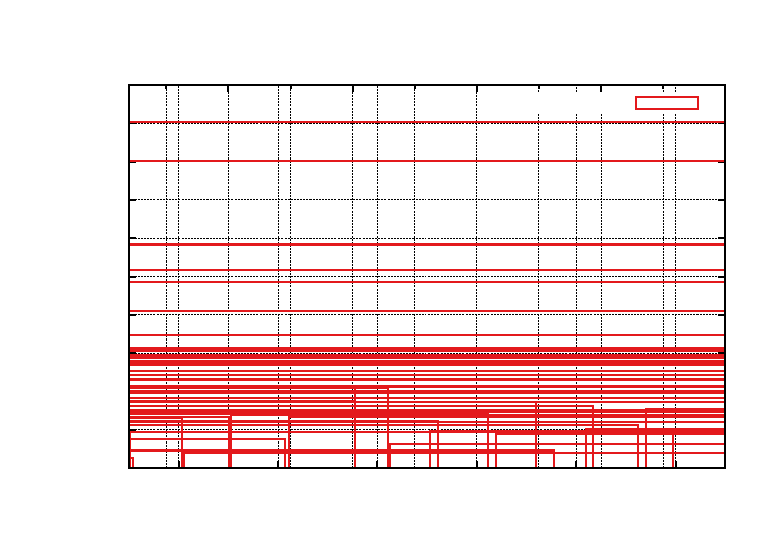
\includegraphics{./plots/langzeitmessung/probe}}%
    \gplfronttext
  \end{picture}%
\endgroup

		}
		\caption{Spektrum der Langzeitmessung nach Abzug des Untergrunds}
		\label{fig:probe_ohne_untergrund}
	\end{subfigure}
	\caption{Subtraktion des gemessenen Untergrundes von dem aufgenommenen Spektrum der Bodenprobe. Anhand der Kalibrierung in \eqref{eq:kalibrierung_halb} wurde für die letzte Grafik auch eine Energieskala zur Abbildung hinzugefügt.}
	\label{fig:langzeitmessung_untergrundabzug}
\end{figure}
An die in dem Spektrum erkennbaren Linien wurde mit Hilfe von \texttt{gnuplot} jeweils eine Gaußfunktion mit konstantem Untergrund (s. auch \eqref{eq:gaussfithypothese}) angepasst.
Durch eine Vergrößerung der Ansicht konnten so insgesamt \num{20} Linien gefunden und angepasst werden.
Die Schwerpunkte dieser Anpassungen sind in Tabelle \ref{tab:langzeitmessung_linien} festgehalten worden. 
Dort wurde ebenfalls auf Grundlage der Kalibrierung \eqref{eq:kalibrierung_halb} eine Umrechung in Energien durchgeführt.
Der Fehler berechnet sich erneut mit Gaußscher Fehlerfortpflanzung zu:
\begin{align}
&\Delta E = \sqrt{n^2 (\Delta m)^2 + m^2 (\Delta n)^2 + (\Delta b)^2} \\
&\text{$m$: Steigung, $b$: Achsenabschnitt der Kalibrierung}\notag
\end{align}
\begin{sidewaystable}[hp]
	\centering
	\begin{tabular}{cSSSSll}
\toprule
Liniennummer & {Schwerpunkt $n$} & {$\Delta n$} & {Energie $E$ / \si{\kilo\electronvolt}} & {$\Delta E$ / \si{\kilo\electronvolt}} & Isotop            & Ursprung               \\ \midrule
1 & 349.21      & 0.25   & 74.72         & 0.07   & \isotope[214]{Bi} & char. Linie (\isotope[214]{Pb}-Zerfall)      \\
2 & 360.37      & 0.31   & 76.96         & 0.08   & \isotope[214]{Bi} & char. Linie (\isotope[214]{Pb}-Zerfall) \\
3 & 397.78      & 0.51   & 84.48         & 0.12   & \isotope[208]{Pb} & char. Linie (\isotope[208]{Pb}-Zerfall) \\
4 & 411.57      & 0.50   & 87.25         & 0.11   & \isotope[208]{Tl} & char. Linie (\isotope[208]{Tl}-Zerfall) \\
5 & 425.15      & 0.61   & 89.98         & 0.14   & --\tablefootnote{Für diesen Energiewert existieren in der Literatur zwei Linien sehr nah beieinander, die hier nicht unterschieden werden können. Bei beiden handelt es sich um jeweils zwei mögliche charakteristische Linien von Bismuth und Thorium.}    			&                          \\
6 & 1165.88     & 0.09   & 238.74        & 0.06   & \isotope[212]{Pb} & \isotope[232]{Th}-Reihe  \\
7 & 1180.69     & 0.71   & 241.72        & 0.15   & \isotope[214]{Pb} & \isotope[238]{U}-Reihe   \\
8 & 1447.45     & 0.16   & 295.29        & 0.06   & \isotope[214]{Pb} & \isotope[238]{U}-Reihe   \\
9 & 1661.98     & 0.17   & 338.38        & 0.06   & \isotope[223]{Ra} / \isotope[228]{Ac} & \isotope[235]{U}-Reihe / \isotope[232]{Th}-Reihe\tablefootnote{In der Literatur liegen auch hier die Zerfallsenergien dieser beiden Isotope so nah beieinander, dass keine eindeutige Identifizierung erfolgen kann.}  \\
10 & 1729.42     & 0.14   & 351.92        & 0.06   & \isotope[214]{Pb} & \isotope[238]{U}-Reihe   \\
11 & 2520.01     & 0.55   & 510.71        & 0.13   & --		            & e$^+$/e$^-$-Annihilierung\\
12 & 2880.60     & 0.18   & 583.13        & 0.07   & \isotope[208]{Tl} & \isotope[232]{Th}-Reihe  \\
13 & 3010.55     & 0.19   & 609.22        & 0.07   & \isotope[214]{Bi} & \isotope[238]{U}-Reihe   \\
14 & 3269.60     & 0.50   & 661.25        & 0.12   & \cs{}             & Reaktorunfall Tschernobyl\\
15 & 3597.50     & 0.53   & 727.11        & 0.13   & \isotope[212]{Bi} & \isotope[232]{Th}-Reihe  \\
16 & 4513.32     & 0.27   & 911.04        & 0.09   & \isotope[228]{Ac} & \isotope[232]{Th}-Reihe  \\
17 & 4779.22     & 1.21   & 964.44        & 0.26   & \isotope[228]{Ac} & \isotope[232]{Th}-Reihe  \\
18 & 4801.32     & 0.45   & 968.88        & 0.12   & \isotope[228]{Ac} & \isotope[232]{Th}-Reihe  \\
19 & 5554.84     & 0.58   & 1120.22       & 0.14   & \isotope[214]{Bi} & \isotope[238]{U}-Reihe   \\
20 & 7249.28     & 0.46   & 1460.53       & 0.13   & \isotope[40]{K}   & Primordial           \\ \bottomrule
\end{tabular}
	\caption{Schwerpunkte (Kanalnummer) der an jede Linie angepassten Gaußfunktionen sowie die mit der Kalibrierung aus \eqref{eq:kalibrierung_halb} berechneten Energien. Außerdem wurden die Isotope mit entsprechenden Zerfallsenergien sowie Ursprünge dieser Isotope dargestellt.}
	\label{tab:langzeitmessung_linien}
\end{sidewaystable}
Mit \cite{gilmore} konnten den jeweiligen Energien der beobachtbaren Linien das zerfallende Isotop zugeordnet werden.
In Abbildung \ref{fig:langzeit_gross} wurde das aufgenommene Spektrum in groß dargestellt und die Liniennummern aus Tabelle \ref{tab:langzeitmessung_linien} den entsprechenden Peaks zugeordnet.
Darüber hinaus wurde in Tabelle \ref{tab:langzeitmessung_linien} ebenfalls der Ursprung der jeweiligen Zerfälle notiert.
Diesen bilden in den meisten Fällen die beiden natürlichen Zerfallsreihen von \isotope[232]{Th} und \isotope[238]{U}, aber auch die \isotope[235]{U}-Zerfallsreihe ist einmal (wenn auch nicht eindeutig, beachte auch die Fußnote) vorhanden.
Weiterhin konnte mit \isotope[40]{K} auch das primordiale Kalium nachgewiesen werden, welches eine der größten Linien im Spektrum darstellt.
Die Anpassungen für niedrige Energien (ca. $<\SI{500}{\kilo\electronvolt}$) gelangen nicht besonders gut, so dass die gefundenen Ursprünge dieser Linien nicht mit großer Sicherheit festgestellt werden konnten.
Dabei handelt es sich in allen Fällen um charakteristische Röntgenlinien der jeweiligen Isotope, die bei den angegebenen Zerfällen entstehen.
Die Mutterkerne gehören jedoch auch immer zu einer natürlichen Zerfallsreihe.
Bei \SI{510.71+-0.13}{\kilo\electronvolt} konnte vermutlich die Annihilierung von Elektronen und Positronen beobachtet werden, die erwartungsgemäß bei \SI{511}{\kilo\electronvolt} stattfindet, mit dem die gefundene Energie gut übereinstimmt.
Außerdem konnte die \cs{}-Linie nachgewiesen werden, die in keiner Zerfallsreihe auftritt.
Bei dem Reaktorunfall von Tschernobyl im Jahr 1986 wurde \cs{} in größeren Mengen freigesetzt und gelangte nach Westeuropa.
Wegen seiner Halbwertszeit von ca. \SI{30}{a} ist es bis heute noch vorhanden, so dass es möglicherweise in der untersuchten Erde beobachtet werden konnte. 
\FloatBarrier

\section{Fazit}

\subsection{Vergleich der Detektoren}
Aufgrund der unterschiedlichen Funktionsweise von Szintillationsdetektor und Halbleiterdetektor ist es nicht verwunderlich, dass diese die beobachteten teilweise unterschiedliche Verhalten zeigen.
In diesem Abschnitt sollen die zuvor experimentell bestimmten Eigenschaften der beiden Detektoren verglichen werden.
\begin{itemize}
	\item \textbf{Signalform:} Beide Detektoren weisen sehr ähnliche Signalformen sowohl am Vor- als auch am Hauptverstärker auf. Sie unterscheiden sich hauptsächlich in Pulsdauer und Höhe.
	
	\item \textbf{Energieauflösung:} Den größten Unterschied der beiden Detektoren stellt man bei dem Auflösungsvermögen fest.
	Eine der Kenngrößen der Auflösung ist die volle Halbwertsbreite (FWHM) der Linien, welche im Falle des Szintillationsdetektors in der Größenordnung von \num{10} bis \SI{100}{keV} liegt.
	Der Halbleiterdetektor weist eine wesentlich größeres Auflösungsvermögen auf, da dessen Halbwertsbreiten zwischen \num{1} und \SI{2}{keV} liegen.
	Diese Tatsache sieht man deutlich in den aufgenommenen Spektren.	
	
	\item \textbf{Peak-to-Total Verhältnis:}
	Das Peak-to-Total Verhältnisses, also die Wahrscheinlichkeit, dass ein detektiertes Quant in den Photopeak fällt, ist für den Szintillationsdetektor um \num{4} bis \SI{6}{\percent} größer als für den verwendeten Halbleiterdetektor.
	
	\item \textbf{Absolute Peakeffizienz:}
	Analog zum vorigen Punkt ist der Szintillationsdetektor auch bei der absoluten Peakeffizienz dem Halbleiterdetektor überlegen.
	Mit dem NaI(Tl)-Szintillator werden \SI{20.1 +- 1.4}{\percent} aller in Richtung des Detektors emittierten $\gamma$-Quanten im Photopeak detektiert.
	Für den Ge-Halbleiterdetektor sind dies lediglich \SI{15.05 +- 0.82}{\percent}.
	
\end{itemize}
Man sieht, dass die Existenz beider Detektortypen gerechtfertigt ist, da beide Detektortypen ihre Vor- und Nachteile haben.
Sollte eine hohe Detektionseffizienz benötigt werden, so könnte ein Szintillationsdetektor für die Aufgabe gut geeignet sein.
Andererseits kann für etwas geringere Effizienz aber mit wesentlich größerer Energieauflösung ein Halbleiterdetektor verwendet werden.

\subsection{Zusammenfassung}
Der durchgeführte Versuch stellt damit zwei gute Detektoren für die Gammaspektroskopie, sowie ein dafür typische Vorgehen in der Auswertung vor.
Diese ist zu großen Teilen gut gelungen, lediglich die Energiekalibrierung des NaI(Tl)-Detektors bzw. die Nichtlinearität des dabei verwendeten Verstärkers fallen dabei störend auf.
Besonders die Berechnung der Halbwertsbreiten ist aus diesem Grund nur bedingt möglich gewesen, so dass die gefundenen Werte keine quantitative Bewertung zulassen.
Die Auswertung für den Halbleiterdetektor ist durchweg erfolgreich gewesen und mit der Energiekalibrierung konnten viele Linien im Spektrum der untersuchten Bodenprobe gefunden und identifiziert werden, die alle plausibel erscheinen und erklärt werden konnten.

\FloatBarrier
% BIBLIOGRAPHIE
\vspace{\fill}
% Maximale Anzahl der Einträge in Klammer
% Zitieren mit \cite{lamport94}
\begin{thebibliography}{19}
\bibitem{siegbahn}
	K. Siegbahn,
	\emph{Alpha-, Beta- and Gamma-Ray Spectroscopy},
	Elsevier Science Ltd. 1965

\bibitem{wermes}
	N. Wermes,
	\emph{physik511: Physik V (Kerne und Teilchen)},
	WS 2014/15

\bibitem{leo}
	W. R. Leo,
	\emph{Techniques for Nuclear and Particle Physics Experiments},
	Springer 1994

\bibitem{anleitung}
	Physikalisches Praktikum V: Kern- und Teilchenphysik,
	Versuchsbeschreibung \emph{P521: $\gamma$-Spektroskopie} (Stand: Januar 2015),
	Universität Bonn	

\bibitem{riezler}
	Riezler, W.; Kopitzki, K.
	\emph{Kernphysikalisches Praktikum},
	Teubner 1963

\bibitem{nist}
	M. P. Unterweger, D. D. Hoppes, F. J. Schima, J.S. Coursey,
	\emph{NIST Radionuclide Half-Life Measurements},
	\url{http://www.nist.gov/pml/data/halflife-html.cfm} (Letzter Abruf: 1. Mai 2015)
	
\bibitem{gilmore}
	Gordon R. Gilmore,
	\emph{Practical Gamma-Ray Spectrometry, 2nd Edition, Appendix D},
	\url{http://onlinelibrary.wiley.com/doi/10.1002/9780470861981.app4/pdf} (Letzter Abruf: 07. Mai 2015)

\end{thebibliography}

% APPENDIX
\begin{appendix}
\section{Anhang}
Auf den folgenden Seiten sind der Vollständigkeit halber alle aufgenommenen Gammaspektren dargestellt.
\begin{figure}[ht]
	\centering
	\begin{subfigure}[b]{0.65\textwidth}
		\resizebox{!}{0.285\textheight}{
			% GNUPLOT: LaTeX picture with Postscript
\begingroup
  \makeatletter
  \providecommand\color[2][]{%
    \GenericError{(gnuplot) \space\space\space\@spaces}{%
      Package color not loaded in conjunction with
      terminal option `colourtext'%
    }{See the gnuplot documentation for explanation.%
    }{Either use 'blacktext' in gnuplot or load the package
      color.sty in LaTeX.}%
    \renewcommand\color[2][]{}%
  }%
  \providecommand\includegraphics[2][]{%
    \GenericError{(gnuplot) \space\space\space\@spaces}{%
      Package graphicx or graphics not loaded%
    }{See the gnuplot documentation for explanation.%
    }{The gnuplot epslatex terminal needs graphicx.sty or graphics.sty.}%
    \renewcommand\includegraphics[2][]{}%
  }%
  \providecommand\rotatebox[2]{#2}%
  \@ifundefined{ifGPcolor}{%
    \newif\ifGPcolor
    \GPcolortrue
  }{}%
  \@ifundefined{ifGPblacktext}{%
    \newif\ifGPblacktext
    \GPblacktexttrue
  }{}%
  % define a \g@addto@macro without @ in the name:
  \let\gplgaddtomacro\g@addto@macro
  % define empty templates for all commands taking text:
  \gdef\gplbacktext{}%
  \gdef\gplfronttext{}%
  \makeatother
  \ifGPblacktext
    % no textcolor at all
    \def\colorrgb#1{}%
    \def\colorgray#1{}%
  \else
    % gray or color?
    \ifGPcolor
      \def\colorrgb#1{\color[rgb]{#1}}%
      \def\colorgray#1{\color[gray]{#1}}%
      \expandafter\def\csname LTw\endcsname{\color{white}}%
      \expandafter\def\csname LTb\endcsname{\color{black}}%
      \expandafter\def\csname LTa\endcsname{\color{black}}%
      \expandafter\def\csname LT0\endcsname{\color[rgb]{1,0,0}}%
      \expandafter\def\csname LT1\endcsname{\color[rgb]{0,1,0}}%
      \expandafter\def\csname LT2\endcsname{\color[rgb]{0,0,1}}%
      \expandafter\def\csname LT3\endcsname{\color[rgb]{1,0,1}}%
      \expandafter\def\csname LT4\endcsname{\color[rgb]{0,1,1}}%
      \expandafter\def\csname LT5\endcsname{\color[rgb]{1,1,0}}%
      \expandafter\def\csname LT6\endcsname{\color[rgb]{0,0,0}}%
      \expandafter\def\csname LT7\endcsname{\color[rgb]{1,0.3,0}}%
      \expandafter\def\csname LT8\endcsname{\color[rgb]{0.5,0.5,0.5}}%
    \else
      % gray
      \def\colorrgb#1{\color{black}}%
      \def\colorgray#1{\color[gray]{#1}}%
      \expandafter\def\csname LTw\endcsname{\color{white}}%
      \expandafter\def\csname LTb\endcsname{\color{black}}%
      \expandafter\def\csname LTa\endcsname{\color{black}}%
      \expandafter\def\csname LT0\endcsname{\color{black}}%
      \expandafter\def\csname LT1\endcsname{\color{black}}%
      \expandafter\def\csname LT2\endcsname{\color{black}}%
      \expandafter\def\csname LT3\endcsname{\color{black}}%
      \expandafter\def\csname LT4\endcsname{\color{black}}%
      \expandafter\def\csname LT5\endcsname{\color{black}}%
      \expandafter\def\csname LT6\endcsname{\color{black}}%
      \expandafter\def\csname LT7\endcsname{\color{black}}%
      \expandafter\def\csname LT8\endcsname{\color{black}}%
    \fi
  \fi
    \setlength{\unitlength}{0.0500bp}%
    \ifx\gptboxheight\undefined%
      \newlength{\gptboxheight}%
      \newlength{\gptboxwidth}%
      \newsavebox{\gptboxtext}%
    \fi%
    \setlength{\fboxrule}{0.5pt}%
    \setlength{\fboxsep}{1pt}%
\begin{picture}(7200.00,5040.00)%
    \gplgaddtomacro\gplbacktext{%
      \csname LTb\endcsname%
      \put(946,704){\makebox(0,0)[r]{\strut{}$0$}}%
      \put(946,1286){\makebox(0,0)[r]{\strut{}$200$}}%
      \put(946,1867){\makebox(0,0)[r]{\strut{}$400$}}%
      \put(946,2449){\makebox(0,0)[r]{\strut{}$600$}}%
      \put(946,3030){\makebox(0,0)[r]{\strut{}$800$}}%
      \put(946,3612){\makebox(0,0)[r]{\strut{}$1000$}}%
      \put(946,4193){\makebox(0,0)[r]{\strut{}$1200$}}%
      \put(946,4775){\makebox(0,0)[r]{\strut{}$1400$}}%
      \put(1078,484){\makebox(0,0){\strut{}$0$}}%
      \put(2223,484){\makebox(0,0){\strut{}$1000$}}%
      \put(3368,484){\makebox(0,0){\strut{}$2000$}}%
      \put(4513,484){\makebox(0,0){\strut{}$3000$}}%
      \put(5658,484){\makebox(0,0){\strut{}$4000$}}%
      \put(6803,484){\makebox(0,0){\strut{}$5000$}}%
      \put(1467,3030){\rotatebox{-270}{\makebox(0,0)[l]{\strut{}Röntgenlinie}}}%
      \put(2371,2914){\rotatebox{-270}{\makebox(0,0)[l]{\strut{}Rückstreupeak}}}%
      \put(4009,1635){\rotatebox{-270}{\makebox(0,0)[l]{\strut{}Compton-Kante}}}%
      \put(5807,3030){\rotatebox{-270}{\makebox(0,0)[l]{\strut{}\SI{661.660}{keV}}}}%
    }%
    \gplgaddtomacro\gplfronttext{%
      \csname LTb\endcsname%
      \put(176,2739){\rotatebox{-270}{\makebox(0,0){\strut{}Ereignisse $N$}}}%
      \put(3940,154){\makebox(0,0){\strut{}Kanal $n$}}%
    }%
    \gplbacktext
    \put(0,0){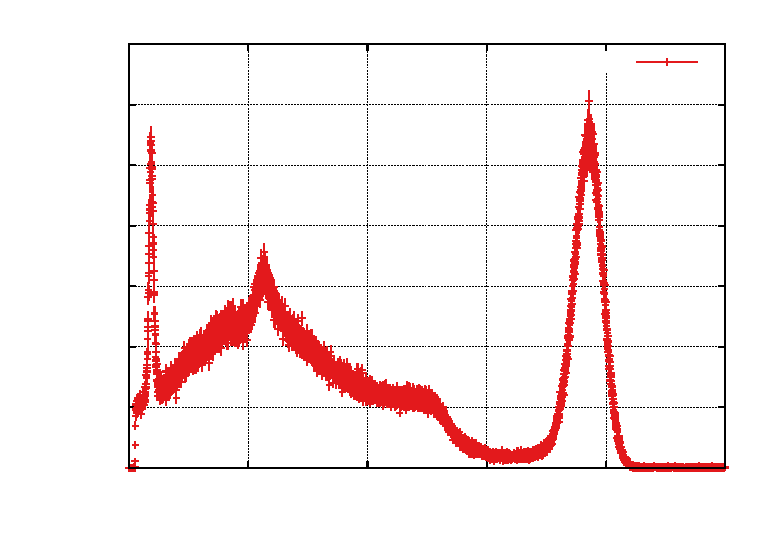
\includegraphics{./plots/szintillator/caesium}}%
    \gplfronttext
  \end{picture}%
\endgroup

		}
		\caption{Gammaspektrum von \cs}
		\label{fig:szin_caesium_spektrum}
	\end{subfigure}
	
	\begin{subfigure}[b]{0.65\textwidth}
		\resizebox{!}{0.285\textheight}{
			% GNUPLOT: LaTeX picture with Postscript
\begingroup
  \makeatletter
  \providecommand\color[2][]{%
    \GenericError{(gnuplot) \space\space\space\@spaces}{%
      Package color not loaded in conjunction with
      terminal option `colourtext'%
    }{See the gnuplot documentation for explanation.%
    }{Either use 'blacktext' in gnuplot or load the package
      color.sty in LaTeX.}%
    \renewcommand\color[2][]{}%
  }%
  \providecommand\includegraphics[2][]{%
    \GenericError{(gnuplot) \space\space\space\@spaces}{%
      Package graphicx or graphics not loaded%
    }{See the gnuplot documentation for explanation.%
    }{The gnuplot epslatex terminal needs graphicx.sty or graphics.sty.}%
    \renewcommand\includegraphics[2][]{}%
  }%
  \providecommand\rotatebox[2]{#2}%
  \@ifundefined{ifGPcolor}{%
    \newif\ifGPcolor
    \GPcolortrue
  }{}%
  \@ifundefined{ifGPblacktext}{%
    \newif\ifGPblacktext
    \GPblacktexttrue
  }{}%
  % define a \g@addto@macro without @ in the name:
  \let\gplgaddtomacro\g@addto@macro
  % define empty templates for all commands taking text:
  \gdef\gplbacktext{}%
  \gdef\gplfronttext{}%
  \makeatother
  \ifGPblacktext
    % no textcolor at all
    \def\colorrgb#1{}%
    \def\colorgray#1{}%
  \else
    % gray or color?
    \ifGPcolor
      \def\colorrgb#1{\color[rgb]{#1}}%
      \def\colorgray#1{\color[gray]{#1}}%
      \expandafter\def\csname LTw\endcsname{\color{white}}%
      \expandafter\def\csname LTb\endcsname{\color{black}}%
      \expandafter\def\csname LTa\endcsname{\color{black}}%
      \expandafter\def\csname LT0\endcsname{\color[rgb]{1,0,0}}%
      \expandafter\def\csname LT1\endcsname{\color[rgb]{0,1,0}}%
      \expandafter\def\csname LT2\endcsname{\color[rgb]{0,0,1}}%
      \expandafter\def\csname LT3\endcsname{\color[rgb]{1,0,1}}%
      \expandafter\def\csname LT4\endcsname{\color[rgb]{0,1,1}}%
      \expandafter\def\csname LT5\endcsname{\color[rgb]{1,1,0}}%
      \expandafter\def\csname LT6\endcsname{\color[rgb]{0,0,0}}%
      \expandafter\def\csname LT7\endcsname{\color[rgb]{1,0.3,0}}%
      \expandafter\def\csname LT8\endcsname{\color[rgb]{0.5,0.5,0.5}}%
    \else
      % gray
      \def\colorrgb#1{\color{black}}%
      \def\colorgray#1{\color[gray]{#1}}%
      \expandafter\def\csname LTw\endcsname{\color{white}}%
      \expandafter\def\csname LTb\endcsname{\color{black}}%
      \expandafter\def\csname LTa\endcsname{\color{black}}%
      \expandafter\def\csname LT0\endcsname{\color{black}}%
      \expandafter\def\csname LT1\endcsname{\color{black}}%
      \expandafter\def\csname LT2\endcsname{\color{black}}%
      \expandafter\def\csname LT3\endcsname{\color{black}}%
      \expandafter\def\csname LT4\endcsname{\color{black}}%
      \expandafter\def\csname LT5\endcsname{\color{black}}%
      \expandafter\def\csname LT6\endcsname{\color{black}}%
      \expandafter\def\csname LT7\endcsname{\color{black}}%
      \expandafter\def\csname LT8\endcsname{\color{black}}%
    \fi
  \fi
    \setlength{\unitlength}{0.0500bp}%
    \ifx\gptboxheight\undefined%
      \newlength{\gptboxheight}%
      \newlength{\gptboxwidth}%
      \newsavebox{\gptboxtext}%
    \fi%
    \setlength{\fboxrule}{0.5pt}%
    \setlength{\fboxsep}{1pt}%
\begin{picture}(7200.00,5040.00)%
    \gplgaddtomacro\gplbacktext{%
      \csname LTb\endcsname%
      \put(946,704){\makebox(0,0)[r]{\strut{}$-100$}}%
      \csname LTb\endcsname%
      \put(946,1074){\makebox(0,0)[r]{\strut{}$0$}}%
      \csname LTb\endcsname%
      \put(946,1444){\makebox(0,0)[r]{\strut{}$100$}}%
      \csname LTb\endcsname%
      \put(946,1814){\makebox(0,0)[r]{\strut{}$200$}}%
      \csname LTb\endcsname%
      \put(946,2184){\makebox(0,0)[r]{\strut{}$300$}}%
      \csname LTb\endcsname%
      \put(946,2554){\makebox(0,0)[r]{\strut{}$400$}}%
      \csname LTb\endcsname%
      \put(946,2925){\makebox(0,0)[r]{\strut{}$500$}}%
      \csname LTb\endcsname%
      \put(946,3295){\makebox(0,0)[r]{\strut{}$600$}}%
      \csname LTb\endcsname%
      \put(946,3665){\makebox(0,0)[r]{\strut{}$700$}}%
      \csname LTb\endcsname%
      \put(946,4035){\makebox(0,0)[r]{\strut{}$800$}}%
      \csname LTb\endcsname%
      \put(946,4405){\makebox(0,0)[r]{\strut{}$900$}}%
      \csname LTb\endcsname%
      \put(946,4775){\makebox(0,0)[r]{\strut{}$1000$}}%
      \csname LTb\endcsname%
      \put(1078,484){\makebox(0,0){\strut{}$-1000$}}%
      \csname LTb\endcsname%
      \put(1651,484){\makebox(0,0){\strut{}$0$}}%
      \csname LTb\endcsname%
      \put(2223,484){\makebox(0,0){\strut{}$1000$}}%
      \csname LTb\endcsname%
      \put(2796,484){\makebox(0,0){\strut{}$2000$}}%
      \csname LTb\endcsname%
      \put(3368,484){\makebox(0,0){\strut{}$3000$}}%
      \csname LTb\endcsname%
      \put(3941,484){\makebox(0,0){\strut{}$4000$}}%
      \csname LTb\endcsname%
      \put(4513,484){\makebox(0,0){\strut{}$5000$}}%
      \csname LTb\endcsname%
      \put(5086,484){\makebox(0,0){\strut{}$6000$}}%
      \csname LTb\endcsname%
      \put(5658,484){\makebox(0,0){\strut{}$7000$}}%
      \csname LTb\endcsname%
      \put(6231,484){\makebox(0,0){\strut{}$8000$}}%
      \csname LTb\endcsname%
      \put(6803,484){\makebox(0,0){\strut{}$9000$}}%
    }%
    \gplgaddtomacro\gplfronttext{%
      \csname LTb\endcsname%
      \put(176,2739){\rotatebox{-270}{\makebox(0,0){\strut{}Ereignisse $$}}}%
      \put(3940,154){\makebox(0,0){\strut{}Kanal $n$}}%
      \csname LTb\endcsname%
      \put(2398,4602){\makebox(0,0)[r]{\strut{}Messwerte}}%
    }%
    \gplbacktext
    \put(0,0){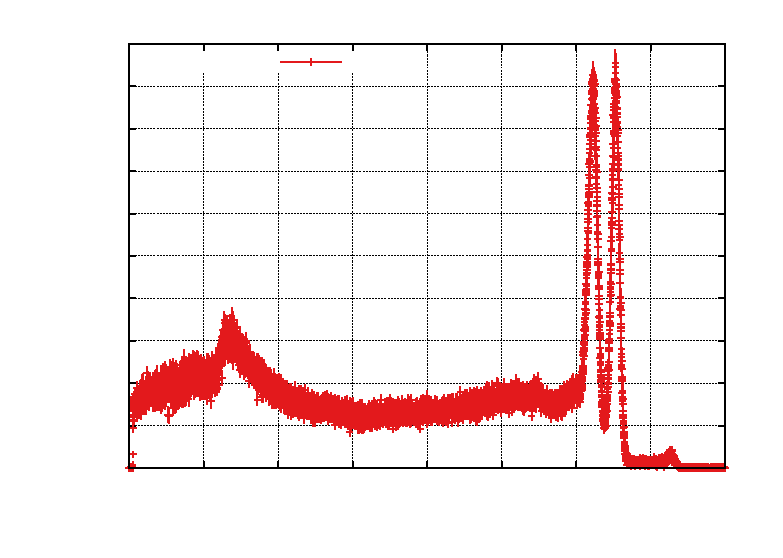
\includegraphics{./plots/szintillator/cobalt}}%
    \gplfronttext
  \end{picture}%
\endgroup

		}
		\caption{Gammaspektrum von \co}
		\label{fig:szin_cobalt_spektrum}
	\end{subfigure}
	
	\begin{subfigure}[b]{0.65\textwidth}
		\resizebox{!}{0.285\textheight}{		
			% GNUPLOT: LaTeX picture with Postscript
\begingroup
  \makeatletter
  \providecommand\color[2][]{%
    \GenericError{(gnuplot) \space\space\space\@spaces}{%
      Package color not loaded in conjunction with
      terminal option `colourtext'%
    }{See the gnuplot documentation for explanation.%
    }{Either use 'blacktext' in gnuplot or load the package
      color.sty in LaTeX.}%
    \renewcommand\color[2][]{}%
  }%
  \providecommand\includegraphics[2][]{%
    \GenericError{(gnuplot) \space\space\space\@spaces}{%
      Package graphicx or graphics not loaded%
    }{See the gnuplot documentation for explanation.%
    }{The gnuplot epslatex terminal needs graphicx.sty or graphics.sty.}%
    \renewcommand\includegraphics[2][]{}%
  }%
  \providecommand\rotatebox[2]{#2}%
  \@ifundefined{ifGPcolor}{%
    \newif\ifGPcolor
    \GPcolortrue
  }{}%
  \@ifundefined{ifGPblacktext}{%
    \newif\ifGPblacktext
    \GPblacktexttrue
  }{}%
  % define a \g@addto@macro without @ in the name:
  \let\gplgaddtomacro\g@addto@macro
  % define empty templates for all commands taking text:
  \gdef\gplbacktext{}%
  \gdef\gplfronttext{}%
  \makeatother
  \ifGPblacktext
    % no textcolor at all
    \def\colorrgb#1{}%
    \def\colorgray#1{}%
  \else
    % gray or color?
    \ifGPcolor
      \def\colorrgb#1{\color[rgb]{#1}}%
      \def\colorgray#1{\color[gray]{#1}}%
      \expandafter\def\csname LTw\endcsname{\color{white}}%
      \expandafter\def\csname LTb\endcsname{\color{black}}%
      \expandafter\def\csname LTa\endcsname{\color{black}}%
      \expandafter\def\csname LT0\endcsname{\color[rgb]{1,0,0}}%
      \expandafter\def\csname LT1\endcsname{\color[rgb]{0,1,0}}%
      \expandafter\def\csname LT2\endcsname{\color[rgb]{0,0,1}}%
      \expandafter\def\csname LT3\endcsname{\color[rgb]{1,0,1}}%
      \expandafter\def\csname LT4\endcsname{\color[rgb]{0,1,1}}%
      \expandafter\def\csname LT5\endcsname{\color[rgb]{1,1,0}}%
      \expandafter\def\csname LT6\endcsname{\color[rgb]{0,0,0}}%
      \expandafter\def\csname LT7\endcsname{\color[rgb]{1,0.3,0}}%
      \expandafter\def\csname LT8\endcsname{\color[rgb]{0.5,0.5,0.5}}%
    \else
      % gray
      \def\colorrgb#1{\color{black}}%
      \def\colorgray#1{\color[gray]{#1}}%
      \expandafter\def\csname LTw\endcsname{\color{white}}%
      \expandafter\def\csname LTb\endcsname{\color{black}}%
      \expandafter\def\csname LTa\endcsname{\color{black}}%
      \expandafter\def\csname LT0\endcsname{\color{black}}%
      \expandafter\def\csname LT1\endcsname{\color{black}}%
      \expandafter\def\csname LT2\endcsname{\color{black}}%
      \expandafter\def\csname LT3\endcsname{\color{black}}%
      \expandafter\def\csname LT4\endcsname{\color{black}}%
      \expandafter\def\csname LT5\endcsname{\color{black}}%
      \expandafter\def\csname LT6\endcsname{\color{black}}%
      \expandafter\def\csname LT7\endcsname{\color{black}}%
      \expandafter\def\csname LT8\endcsname{\color{black}}%
    \fi
  \fi
    \setlength{\unitlength}{0.0500bp}%
    \ifx\gptboxheight\undefined%
      \newlength{\gptboxheight}%
      \newlength{\gptboxwidth}%
      \newsavebox{\gptboxtext}%
    \fi%
    \setlength{\fboxrule}{0.5pt}%
    \setlength{\fboxsep}{1pt}%
\begin{picture}(7200.00,5040.00)%
    \gplgaddtomacro\gplbacktext{%
      \csname LTb\endcsname%
      \put(1078,704){\makebox(0,0)[r]{\strut{}$0$}}%
      \put(1078,1383){\makebox(0,0)[r]{\strut{}$5000$}}%
      \put(1078,2061){\makebox(0,0)[r]{\strut{}$10000$}}%
      \put(1078,2740){\makebox(0,0)[r]{\strut{}$15000$}}%
      \put(1078,3418){\makebox(0,0)[r]{\strut{}$20000$}}%
      \put(1078,4097){\makebox(0,0)[r]{\strut{}$25000$}}%
      \put(1078,4775){\makebox(0,0)[r]{\strut{}$30000$}}%
      \put(1210,484){\makebox(0,0){\strut{}$0$}}%
      \put(1909,484){\makebox(0,0){\strut{}$1000$}}%
      \put(2608,484){\makebox(0,0){\strut{}$2000$}}%
      \put(3307,484){\makebox(0,0){\strut{}$3000$}}%
      \put(4007,484){\makebox(0,0){\strut{}$4000$}}%
      \put(4706,484){\makebox(0,0){\strut{}$5000$}}%
      \put(5405,484){\makebox(0,0){\strut{}$6000$}}%
      \put(6104,484){\makebox(0,0){\strut{}$7000$}}%
      \put(6803,484){\makebox(0,0){\strut{}$8000$}}%
      \put(4908,1005){\rotatebox{-270}{\makebox(0,0)[l]{\strut{}\SI{1085.914}{keV}}}}%
      \put(1748,3011){\rotatebox{-270}{\makebox(0,0)[l]{\strut{}\SI{121.783}{keV}}}}%
      \put(2047,1569){\rotatebox{-270}{\makebox(0,0)[l]{\strut{}\SI{244.699}{keV}}}}%
      \put(2392,2427){\rotatebox{-270}{\makebox(0,0)[l]{\strut{}\SI{344.281}{keV}}}}%
      \put(3916,1089){\rotatebox{-270}{\makebox(0,0)[l]{\strut{}\SI{778.903}{keV}}}}%
      \put(4554,1051){\rotatebox{-270}{\makebox(0,0)[l]{\strut{}\SI{964.131}{keV}}}}%
      \put(5125,1005){\rotatebox{-270}{\makebox(0,0)[l]{\strut{}\SI{1112.116}{keV}}}}%
      \put(6104,1024){\rotatebox{-270}{\makebox(0,0)[l]{\strut{}\SI{1408.011}{keV}}}}%
    }%
    \gplgaddtomacro\gplfronttext{%
      \csname LTb\endcsname%
      \put(176,2739){\rotatebox{-270}{\makebox(0,0){\strut{}Ereignisse $N$}}}%
      \put(4006,154){\makebox(0,0){\strut{}Kanal $n$}}%
    }%
    \gplbacktext
    \put(0,0){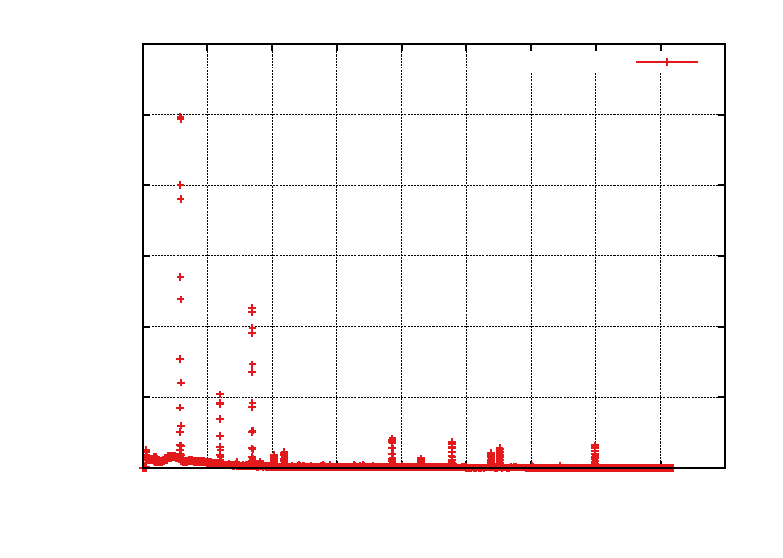
\includegraphics{./plots/halbleiter/europium}}%
    \gplfronttext
  \end{picture}%
\endgroup

		}
		\caption{Gammaspektrum von \isotope[152]{Eu}}
		\label{fig:szin_europium_spektrum}
	\end{subfigure}
	\caption{Übersicht über die um den Untergrund korrigierten Spektren, die mit dem NaI(Tl)-Szintillationsdetektor aufgenommen wurden. Die Messzeit betrug jeweils \SI{720}{\second}.}
\end{figure}

\begin{figure}[ht]
	\centering
	\begin{subfigure}[b]{0.65\textwidth}
		\resizebox{!}{0.285\textheight}{
			% GNUPLOT: LaTeX picture with Postscript
\begingroup
  \makeatletter
  \providecommand\color[2][]{%
    \GenericError{(gnuplot) \space\space\space\@spaces}{%
      Package color not loaded in conjunction with
      terminal option `colourtext'%
    }{See the gnuplot documentation for explanation.%
    }{Either use 'blacktext' in gnuplot or load the package
      color.sty in LaTeX.}%
    \renewcommand\color[2][]{}%
  }%
  \providecommand\includegraphics[2][]{%
    \GenericError{(gnuplot) \space\space\space\@spaces}{%
      Package graphicx or graphics not loaded%
    }{See the gnuplot documentation for explanation.%
    }{The gnuplot epslatex terminal needs graphicx.sty or graphics.sty.}%
    \renewcommand\includegraphics[2][]{}%
  }%
  \providecommand\rotatebox[2]{#2}%
  \@ifundefined{ifGPcolor}{%
    \newif\ifGPcolor
    \GPcolortrue
  }{}%
  \@ifundefined{ifGPblacktext}{%
    \newif\ifGPblacktext
    \GPblacktexttrue
  }{}%
  % define a \g@addto@macro without @ in the name:
  \let\gplgaddtomacro\g@addto@macro
  % define empty templates for all commands taking text:
  \gdef\gplbacktext{}%
  \gdef\gplfronttext{}%
  \makeatother
  \ifGPblacktext
    % no textcolor at all
    \def\colorrgb#1{}%
    \def\colorgray#1{}%
  \else
    % gray or color?
    \ifGPcolor
      \def\colorrgb#1{\color[rgb]{#1}}%
      \def\colorgray#1{\color[gray]{#1}}%
      \expandafter\def\csname LTw\endcsname{\color{white}}%
      \expandafter\def\csname LTb\endcsname{\color{black}}%
      \expandafter\def\csname LTa\endcsname{\color{black}}%
      \expandafter\def\csname LT0\endcsname{\color[rgb]{1,0,0}}%
      \expandafter\def\csname LT1\endcsname{\color[rgb]{0,1,0}}%
      \expandafter\def\csname LT2\endcsname{\color[rgb]{0,0,1}}%
      \expandafter\def\csname LT3\endcsname{\color[rgb]{1,0,1}}%
      \expandafter\def\csname LT4\endcsname{\color[rgb]{0,1,1}}%
      \expandafter\def\csname LT5\endcsname{\color[rgb]{1,1,0}}%
      \expandafter\def\csname LT6\endcsname{\color[rgb]{0,0,0}}%
      \expandafter\def\csname LT7\endcsname{\color[rgb]{1,0.3,0}}%
      \expandafter\def\csname LT8\endcsname{\color[rgb]{0.5,0.5,0.5}}%
    \else
      % gray
      \def\colorrgb#1{\color{black}}%
      \def\colorgray#1{\color[gray]{#1}}%
      \expandafter\def\csname LTw\endcsname{\color{white}}%
      \expandafter\def\csname LTb\endcsname{\color{black}}%
      \expandafter\def\csname LTa\endcsname{\color{black}}%
      \expandafter\def\csname LT0\endcsname{\color{black}}%
      \expandafter\def\csname LT1\endcsname{\color{black}}%
      \expandafter\def\csname LT2\endcsname{\color{black}}%
      \expandafter\def\csname LT3\endcsname{\color{black}}%
      \expandafter\def\csname LT4\endcsname{\color{black}}%
      \expandafter\def\csname LT5\endcsname{\color{black}}%
      \expandafter\def\csname LT6\endcsname{\color{black}}%
      \expandafter\def\csname LT7\endcsname{\color{black}}%
      \expandafter\def\csname LT8\endcsname{\color{black}}%
    \fi
  \fi
    \setlength{\unitlength}{0.0500bp}%
    \ifx\gptboxheight\undefined%
      \newlength{\gptboxheight}%
      \newlength{\gptboxwidth}%
      \newsavebox{\gptboxtext}%
    \fi%
    \setlength{\fboxrule}{0.5pt}%
    \setlength{\fboxsep}{1pt}%
\begin{picture}(7200.00,5040.00)%
    \gplgaddtomacro\gplbacktext{%
      \csname LTb\endcsname%
      \put(946,704){\makebox(0,0)[r]{\strut{}$0$}}%
      \put(946,1286){\makebox(0,0)[r]{\strut{}$200$}}%
      \put(946,1867){\makebox(0,0)[r]{\strut{}$400$}}%
      \put(946,2449){\makebox(0,0)[r]{\strut{}$600$}}%
      \put(946,3030){\makebox(0,0)[r]{\strut{}$800$}}%
      \put(946,3612){\makebox(0,0)[r]{\strut{}$1000$}}%
      \put(946,4193){\makebox(0,0)[r]{\strut{}$1200$}}%
      \put(946,4775){\makebox(0,0)[r]{\strut{}$1400$}}%
      \put(1078,484){\makebox(0,0){\strut{}$0$}}%
      \put(2223,484){\makebox(0,0){\strut{}$1000$}}%
      \put(3368,484){\makebox(0,0){\strut{}$2000$}}%
      \put(4513,484){\makebox(0,0){\strut{}$3000$}}%
      \put(5658,484){\makebox(0,0){\strut{}$4000$}}%
      \put(6803,484){\makebox(0,0){\strut{}$5000$}}%
      \put(1467,3030){\rotatebox{-270}{\makebox(0,0)[l]{\strut{}Röntgenlinie}}}%
      \put(2371,2914){\rotatebox{-270}{\makebox(0,0)[l]{\strut{}Rückstreupeak}}}%
      \put(4009,1635){\rotatebox{-270}{\makebox(0,0)[l]{\strut{}Compton-Kante}}}%
      \put(5807,3030){\rotatebox{-270}{\makebox(0,0)[l]{\strut{}\SI{661.660}{keV}}}}%
    }%
    \gplgaddtomacro\gplfronttext{%
      \csname LTb\endcsname%
      \put(176,2739){\rotatebox{-270}{\makebox(0,0){\strut{}Ereignisse $N$}}}%
      \put(3940,154){\makebox(0,0){\strut{}Kanal $n$}}%
    }%
    \gplbacktext
    \put(0,0){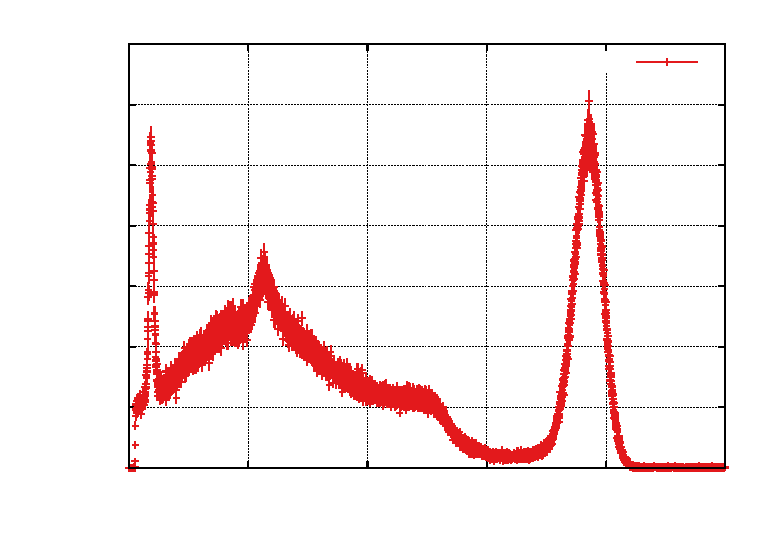
\includegraphics{./plots/szintillator/caesium}}%
    \gplfronttext
  \end{picture}%
\endgroup

		}
		\caption{Gammaspektrum von \cs}
		\label{fig:halb_caesium_spektrum}
	\end{subfigure}
	
	\begin{subfigure}[b]{0.65\textwidth}
		\resizebox{!}{0.285\textheight}{
			% GNUPLOT: LaTeX picture with Postscript
\begingroup
  \makeatletter
  \providecommand\color[2][]{%
    \GenericError{(gnuplot) \space\space\space\@spaces}{%
      Package color not loaded in conjunction with
      terminal option `colourtext'%
    }{See the gnuplot documentation for explanation.%
    }{Either use 'blacktext' in gnuplot or load the package
      color.sty in LaTeX.}%
    \renewcommand\color[2][]{}%
  }%
  \providecommand\includegraphics[2][]{%
    \GenericError{(gnuplot) \space\space\space\@spaces}{%
      Package graphicx or graphics not loaded%
    }{See the gnuplot documentation for explanation.%
    }{The gnuplot epslatex terminal needs graphicx.sty or graphics.sty.}%
    \renewcommand\includegraphics[2][]{}%
  }%
  \providecommand\rotatebox[2]{#2}%
  \@ifundefined{ifGPcolor}{%
    \newif\ifGPcolor
    \GPcolortrue
  }{}%
  \@ifundefined{ifGPblacktext}{%
    \newif\ifGPblacktext
    \GPblacktexttrue
  }{}%
  % define a \g@addto@macro without @ in the name:
  \let\gplgaddtomacro\g@addto@macro
  % define empty templates for all commands taking text:
  \gdef\gplbacktext{}%
  \gdef\gplfronttext{}%
  \makeatother
  \ifGPblacktext
    % no textcolor at all
    \def\colorrgb#1{}%
    \def\colorgray#1{}%
  \else
    % gray or color?
    \ifGPcolor
      \def\colorrgb#1{\color[rgb]{#1}}%
      \def\colorgray#1{\color[gray]{#1}}%
      \expandafter\def\csname LTw\endcsname{\color{white}}%
      \expandafter\def\csname LTb\endcsname{\color{black}}%
      \expandafter\def\csname LTa\endcsname{\color{black}}%
      \expandafter\def\csname LT0\endcsname{\color[rgb]{1,0,0}}%
      \expandafter\def\csname LT1\endcsname{\color[rgb]{0,1,0}}%
      \expandafter\def\csname LT2\endcsname{\color[rgb]{0,0,1}}%
      \expandafter\def\csname LT3\endcsname{\color[rgb]{1,0,1}}%
      \expandafter\def\csname LT4\endcsname{\color[rgb]{0,1,1}}%
      \expandafter\def\csname LT5\endcsname{\color[rgb]{1,1,0}}%
      \expandafter\def\csname LT6\endcsname{\color[rgb]{0,0,0}}%
      \expandafter\def\csname LT7\endcsname{\color[rgb]{1,0.3,0}}%
      \expandafter\def\csname LT8\endcsname{\color[rgb]{0.5,0.5,0.5}}%
    \else
      % gray
      \def\colorrgb#1{\color{black}}%
      \def\colorgray#1{\color[gray]{#1}}%
      \expandafter\def\csname LTw\endcsname{\color{white}}%
      \expandafter\def\csname LTb\endcsname{\color{black}}%
      \expandafter\def\csname LTa\endcsname{\color{black}}%
      \expandafter\def\csname LT0\endcsname{\color{black}}%
      \expandafter\def\csname LT1\endcsname{\color{black}}%
      \expandafter\def\csname LT2\endcsname{\color{black}}%
      \expandafter\def\csname LT3\endcsname{\color{black}}%
      \expandafter\def\csname LT4\endcsname{\color{black}}%
      \expandafter\def\csname LT5\endcsname{\color{black}}%
      \expandafter\def\csname LT6\endcsname{\color{black}}%
      \expandafter\def\csname LT7\endcsname{\color{black}}%
      \expandafter\def\csname LT8\endcsname{\color{black}}%
    \fi
  \fi
    \setlength{\unitlength}{0.0500bp}%
    \ifx\gptboxheight\undefined%
      \newlength{\gptboxheight}%
      \newlength{\gptboxwidth}%
      \newsavebox{\gptboxtext}%
    \fi%
    \setlength{\fboxrule}{0.5pt}%
    \setlength{\fboxsep}{1pt}%
\begin{picture}(7200.00,5040.00)%
    \gplgaddtomacro\gplbacktext{%
      \csname LTb\endcsname%
      \put(946,704){\makebox(0,0)[r]{\strut{}$-100$}}%
      \csname LTb\endcsname%
      \put(946,1074){\makebox(0,0)[r]{\strut{}$0$}}%
      \csname LTb\endcsname%
      \put(946,1444){\makebox(0,0)[r]{\strut{}$100$}}%
      \csname LTb\endcsname%
      \put(946,1814){\makebox(0,0)[r]{\strut{}$200$}}%
      \csname LTb\endcsname%
      \put(946,2184){\makebox(0,0)[r]{\strut{}$300$}}%
      \csname LTb\endcsname%
      \put(946,2554){\makebox(0,0)[r]{\strut{}$400$}}%
      \csname LTb\endcsname%
      \put(946,2925){\makebox(0,0)[r]{\strut{}$500$}}%
      \csname LTb\endcsname%
      \put(946,3295){\makebox(0,0)[r]{\strut{}$600$}}%
      \csname LTb\endcsname%
      \put(946,3665){\makebox(0,0)[r]{\strut{}$700$}}%
      \csname LTb\endcsname%
      \put(946,4035){\makebox(0,0)[r]{\strut{}$800$}}%
      \csname LTb\endcsname%
      \put(946,4405){\makebox(0,0)[r]{\strut{}$900$}}%
      \csname LTb\endcsname%
      \put(946,4775){\makebox(0,0)[r]{\strut{}$1000$}}%
      \csname LTb\endcsname%
      \put(1078,484){\makebox(0,0){\strut{}$-1000$}}%
      \csname LTb\endcsname%
      \put(1651,484){\makebox(0,0){\strut{}$0$}}%
      \csname LTb\endcsname%
      \put(2223,484){\makebox(0,0){\strut{}$1000$}}%
      \csname LTb\endcsname%
      \put(2796,484){\makebox(0,0){\strut{}$2000$}}%
      \csname LTb\endcsname%
      \put(3368,484){\makebox(0,0){\strut{}$3000$}}%
      \csname LTb\endcsname%
      \put(3941,484){\makebox(0,0){\strut{}$4000$}}%
      \csname LTb\endcsname%
      \put(4513,484){\makebox(0,0){\strut{}$5000$}}%
      \csname LTb\endcsname%
      \put(5086,484){\makebox(0,0){\strut{}$6000$}}%
      \csname LTb\endcsname%
      \put(5658,484){\makebox(0,0){\strut{}$7000$}}%
      \csname LTb\endcsname%
      \put(6231,484){\makebox(0,0){\strut{}$8000$}}%
      \csname LTb\endcsname%
      \put(6803,484){\makebox(0,0){\strut{}$9000$}}%
    }%
    \gplgaddtomacro\gplfronttext{%
      \csname LTb\endcsname%
      \put(176,2739){\rotatebox{-270}{\makebox(0,0){\strut{}Ereignisse $$}}}%
      \put(3940,154){\makebox(0,0){\strut{}Kanal $n$}}%
      \csname LTb\endcsname%
      \put(2398,4602){\makebox(0,0)[r]{\strut{}Messwerte}}%
    }%
    \gplbacktext
    \put(0,0){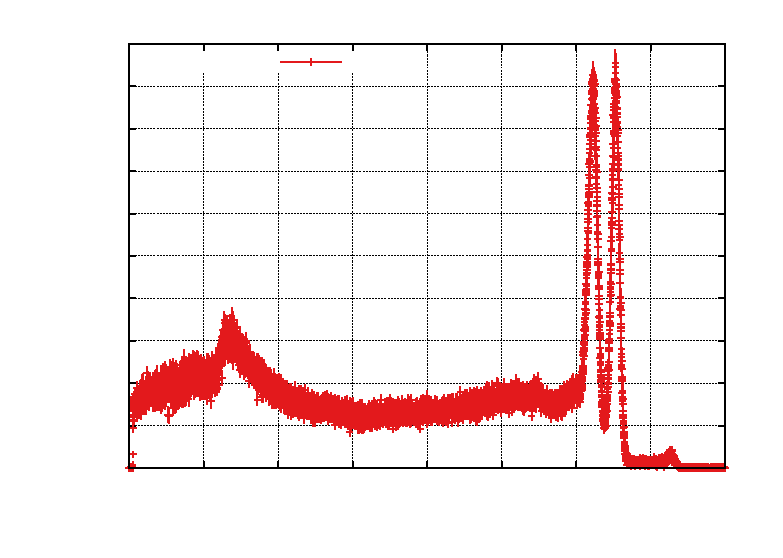
\includegraphics{./plots/szintillator/cobalt}}%
    \gplfronttext
  \end{picture}%
\endgroup

		}
		\caption{Gammaspektrum von \co}
		\label{fig:halb_cobalt_spektrum}
	\end{subfigure}
	
	\begin{subfigure}[b]{0.65\textwidth}
		\resizebox{!}{0.285\textheight}{
	% GNUPLOT: LaTeX picture with Postscript
\begingroup
  \makeatletter
  \providecommand\color[2][]{%
    \GenericError{(gnuplot) \space\space\space\@spaces}{%
      Package color not loaded in conjunction with
      terminal option `colourtext'%
    }{See the gnuplot documentation for explanation.%
    }{Either use 'blacktext' in gnuplot or load the package
      color.sty in LaTeX.}%
    \renewcommand\color[2][]{}%
  }%
  \providecommand\includegraphics[2][]{%
    \GenericError{(gnuplot) \space\space\space\@spaces}{%
      Package graphicx or graphics not loaded%
    }{See the gnuplot documentation for explanation.%
    }{The gnuplot epslatex terminal needs graphicx.sty or graphics.sty.}%
    \renewcommand\includegraphics[2][]{}%
  }%
  \providecommand\rotatebox[2]{#2}%
  \@ifundefined{ifGPcolor}{%
    \newif\ifGPcolor
    \GPcolortrue
  }{}%
  \@ifundefined{ifGPblacktext}{%
    \newif\ifGPblacktext
    \GPblacktexttrue
  }{}%
  % define a \g@addto@macro without @ in the name:
  \let\gplgaddtomacro\g@addto@macro
  % define empty templates for all commands taking text:
  \gdef\gplbacktext{}%
  \gdef\gplfronttext{}%
  \makeatother
  \ifGPblacktext
    % no textcolor at all
    \def\colorrgb#1{}%
    \def\colorgray#1{}%
  \else
    % gray or color?
    \ifGPcolor
      \def\colorrgb#1{\color[rgb]{#1}}%
      \def\colorgray#1{\color[gray]{#1}}%
      \expandafter\def\csname LTw\endcsname{\color{white}}%
      \expandafter\def\csname LTb\endcsname{\color{black}}%
      \expandafter\def\csname LTa\endcsname{\color{black}}%
      \expandafter\def\csname LT0\endcsname{\color[rgb]{1,0,0}}%
      \expandafter\def\csname LT1\endcsname{\color[rgb]{0,1,0}}%
      \expandafter\def\csname LT2\endcsname{\color[rgb]{0,0,1}}%
      \expandafter\def\csname LT3\endcsname{\color[rgb]{1,0,1}}%
      \expandafter\def\csname LT4\endcsname{\color[rgb]{0,1,1}}%
      \expandafter\def\csname LT5\endcsname{\color[rgb]{1,1,0}}%
      \expandafter\def\csname LT6\endcsname{\color[rgb]{0,0,0}}%
      \expandafter\def\csname LT7\endcsname{\color[rgb]{1,0.3,0}}%
      \expandafter\def\csname LT8\endcsname{\color[rgb]{0.5,0.5,0.5}}%
    \else
      % gray
      \def\colorrgb#1{\color{black}}%
      \def\colorgray#1{\color[gray]{#1}}%
      \expandafter\def\csname LTw\endcsname{\color{white}}%
      \expandafter\def\csname LTb\endcsname{\color{black}}%
      \expandafter\def\csname LTa\endcsname{\color{black}}%
      \expandafter\def\csname LT0\endcsname{\color{black}}%
      \expandafter\def\csname LT1\endcsname{\color{black}}%
      \expandafter\def\csname LT2\endcsname{\color{black}}%
      \expandafter\def\csname LT3\endcsname{\color{black}}%
      \expandafter\def\csname LT4\endcsname{\color{black}}%
      \expandafter\def\csname LT5\endcsname{\color{black}}%
      \expandafter\def\csname LT6\endcsname{\color{black}}%
      \expandafter\def\csname LT7\endcsname{\color{black}}%
      \expandafter\def\csname LT8\endcsname{\color{black}}%
    \fi
  \fi
    \setlength{\unitlength}{0.0500bp}%
    \ifx\gptboxheight\undefined%
      \newlength{\gptboxheight}%
      \newlength{\gptboxwidth}%
      \newsavebox{\gptboxtext}%
    \fi%
    \setlength{\fboxrule}{0.5pt}%
    \setlength{\fboxsep}{1pt}%
\begin{picture}(7200.00,5040.00)%
    \gplgaddtomacro\gplbacktext{%
      \csname LTb\endcsname%
      \put(1078,704){\makebox(0,0)[r]{\strut{}$0$}}%
      \put(1078,1383){\makebox(0,0)[r]{\strut{}$5000$}}%
      \put(1078,2061){\makebox(0,0)[r]{\strut{}$10000$}}%
      \put(1078,2740){\makebox(0,0)[r]{\strut{}$15000$}}%
      \put(1078,3418){\makebox(0,0)[r]{\strut{}$20000$}}%
      \put(1078,4097){\makebox(0,0)[r]{\strut{}$25000$}}%
      \put(1078,4775){\makebox(0,0)[r]{\strut{}$30000$}}%
      \put(1210,484){\makebox(0,0){\strut{}$0$}}%
      \put(1909,484){\makebox(0,0){\strut{}$1000$}}%
      \put(2608,484){\makebox(0,0){\strut{}$2000$}}%
      \put(3307,484){\makebox(0,0){\strut{}$3000$}}%
      \put(4007,484){\makebox(0,0){\strut{}$4000$}}%
      \put(4706,484){\makebox(0,0){\strut{}$5000$}}%
      \put(5405,484){\makebox(0,0){\strut{}$6000$}}%
      \put(6104,484){\makebox(0,0){\strut{}$7000$}}%
      \put(6803,484){\makebox(0,0){\strut{}$8000$}}%
      \put(4908,1005){\rotatebox{-270}{\makebox(0,0)[l]{\strut{}\SI{1085.914}{keV}}}}%
      \put(1748,3011){\rotatebox{-270}{\makebox(0,0)[l]{\strut{}\SI{121.783}{keV}}}}%
      \put(2047,1569){\rotatebox{-270}{\makebox(0,0)[l]{\strut{}\SI{244.699}{keV}}}}%
      \put(2392,2427){\rotatebox{-270}{\makebox(0,0)[l]{\strut{}\SI{344.281}{keV}}}}%
      \put(3916,1089){\rotatebox{-270}{\makebox(0,0)[l]{\strut{}\SI{778.903}{keV}}}}%
      \put(4554,1051){\rotatebox{-270}{\makebox(0,0)[l]{\strut{}\SI{964.131}{keV}}}}%
      \put(5125,1005){\rotatebox{-270}{\makebox(0,0)[l]{\strut{}\SI{1112.116}{keV}}}}%
      \put(6104,1024){\rotatebox{-270}{\makebox(0,0)[l]{\strut{}\SI{1408.011}{keV}}}}%
    }%
    \gplgaddtomacro\gplfronttext{%
      \csname LTb\endcsname%
      \put(176,2739){\rotatebox{-270}{\makebox(0,0){\strut{}Ereignisse $N$}}}%
      \put(4006,154){\makebox(0,0){\strut{}Kanal $n$}}%
    }%
    \gplbacktext
    \put(0,0){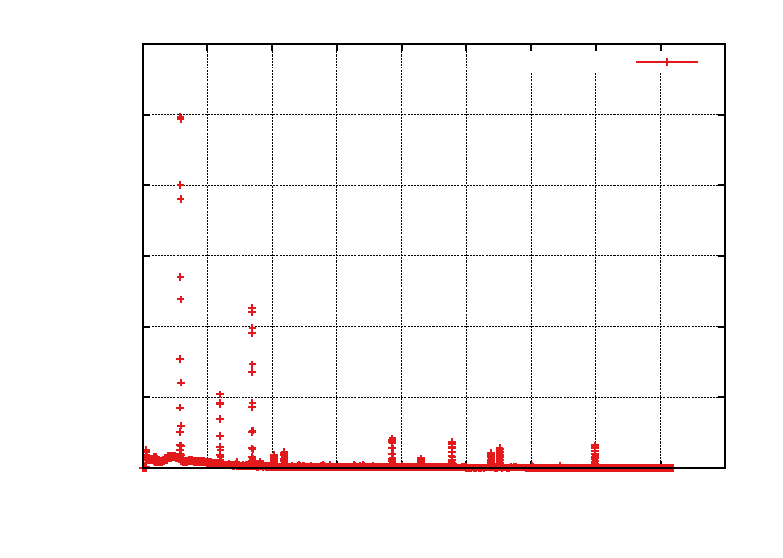
\includegraphics{./plots/halbleiter/europium}}%
    \gplfronttext
  \end{picture}%
\endgroup

	}
	\caption{Gammaspektrum von \isotope[152]{Eu}}
	\label{fig:halb_europium_spektrum}
	\end{subfigure}
	\caption{Übersicht über die um den Untergrund korrigierten Spektren, die mit dem Ge-Halbleiterdetektor aufgenommen wurden. Die Messzeit betrug jeweils \SI{720}{\second}.}
\end{figure}

\begin{sidewaysfigure}
		\centering
		% GNUPLOT: LaTeX picture with Postscript
\begingroup
  \makeatletter
  \providecommand\color[2][]{%
    \GenericError{(gnuplot) \space\space\space\@spaces}{%
      Package color not loaded in conjunction with
      terminal option `colourtext'%
    }{See the gnuplot documentation for explanation.%
    }{Either use 'blacktext' in gnuplot or load the package
      color.sty in LaTeX.}%
    \renewcommand\color[2][]{}%
  }%
  \providecommand\includegraphics[2][]{%
    \GenericError{(gnuplot) \space\space\space\@spaces}{%
      Package graphicx or graphics not loaded%
    }{See the gnuplot documentation for explanation.%
    }{The gnuplot epslatex terminal needs graphicx.sty or graphics.sty.}%
    \renewcommand\includegraphics[2][]{}%
  }%
  \providecommand\rotatebox[2]{#2}%
  \@ifundefined{ifGPcolor}{%
    \newif\ifGPcolor
    \GPcolortrue
  }{}%
  \@ifundefined{ifGPblacktext}{%
    \newif\ifGPblacktext
    \GPblacktexttrue
  }{}%
  % define a \g@addto@macro without @ in the name:
  \let\gplgaddtomacro\g@addto@macro
  % define empty templates for all commands taking text:
  \gdef\gplbacktext{}%
  \gdef\gplfronttext{}%
  \makeatother
  \ifGPblacktext
    % no textcolor at all
    \def\colorrgb#1{}%
    \def\colorgray#1{}%
  \else
    % gray or color?
    \ifGPcolor
      \def\colorrgb#1{\color[rgb]{#1}}%
      \def\colorgray#1{\color[gray]{#1}}%
      \expandafter\def\csname LTw\endcsname{\color{white}}%
      \expandafter\def\csname LTb\endcsname{\color{black}}%
      \expandafter\def\csname LTa\endcsname{\color{black}}%
      \expandafter\def\csname LT0\endcsname{\color[rgb]{1,0,0}}%
      \expandafter\def\csname LT1\endcsname{\color[rgb]{0,1,0}}%
      \expandafter\def\csname LT2\endcsname{\color[rgb]{0,0,1}}%
      \expandafter\def\csname LT3\endcsname{\color[rgb]{1,0,1}}%
      \expandafter\def\csname LT4\endcsname{\color[rgb]{0,1,1}}%
      \expandafter\def\csname LT5\endcsname{\color[rgb]{1,1,0}}%
      \expandafter\def\csname LT6\endcsname{\color[rgb]{0,0,0}}%
      \expandafter\def\csname LT7\endcsname{\color[rgb]{1,0.3,0}}%
      \expandafter\def\csname LT8\endcsname{\color[rgb]{0.5,0.5,0.5}}%
    \else
      % gray
      \def\colorrgb#1{\color{black}}%
      \def\colorgray#1{\color[gray]{#1}}%
      \expandafter\def\csname LTw\endcsname{\color{white}}%
      \expandafter\def\csname LTb\endcsname{\color{black}}%
      \expandafter\def\csname LTa\endcsname{\color{black}}%
      \expandafter\def\csname LT0\endcsname{\color{black}}%
      \expandafter\def\csname LT1\endcsname{\color{black}}%
      \expandafter\def\csname LT2\endcsname{\color{black}}%
      \expandafter\def\csname LT3\endcsname{\color{black}}%
      \expandafter\def\csname LT4\endcsname{\color{black}}%
      \expandafter\def\csname LT5\endcsname{\color{black}}%
      \expandafter\def\csname LT6\endcsname{\color{black}}%
      \expandafter\def\csname LT7\endcsname{\color{black}}%
      \expandafter\def\csname LT8\endcsname{\color{black}}%
    \fi
  \fi
    \setlength{\unitlength}{0.0500bp}%
    \ifx\gptboxheight\undefined%
      \newlength{\gptboxheight}%
      \newlength{\gptboxwidth}%
      \newsavebox{\gptboxtext}%
    \fi%
    \setlength{\fboxrule}{0.5pt}%
    \setlength{\fboxsep}{1pt}%
\begin{picture}(11520.00,8062.00)%
    \gplgaddtomacro\gplbacktext{%
      \csname LTb\endcsname%
      \put(946,704){\makebox(0,0)[r]{\strut{}$0$}}%
      \csname LTb\endcsname%
      \put(946,1820){\makebox(0,0)[r]{\strut{}$200$}}%
      \csname LTb\endcsname%
      \put(946,2936){\makebox(0,0)[r]{\strut{}$400$}}%
      \csname LTb\endcsname%
      \put(946,4053){\makebox(0,0)[r]{\strut{}$600$}}%
      \csname LTb\endcsname%
      \put(946,5169){\makebox(0,0)[r]{\strut{}$800$}}%
      \csname LTb\endcsname%
      \put(946,6285){\makebox(0,0)[r]{\strut{}$1000$}}%
      \csname LTb\endcsname%
      \put(946,7401){\makebox(0,0)[r]{\strut{}$1200$}}%
      \put(2333,484){\makebox(0,0){\strut{}$1000$}}%
      \put(3588,484){\makebox(0,0){\strut{}$2000$}}%
      \put(4844,484){\makebox(0,0){\strut{}$3000$}}%
      \put(6100,484){\makebox(0,0){\strut{}$4000$}}%
      \put(7356,484){\makebox(0,0){\strut{}$5000$}}%
      \put(8611,484){\makebox(0,0){\strut{}$6000$}}%
      \put(9867,484){\makebox(0,0){\strut{}$7000$}}%
      \put(11123,484){\makebox(0,0){\strut{}$8000$}}%
      \csname LTb\endcsname%
      \put(2299,7621){\makebox(0,0){\strut{}$200$}}%
      \csname LTb\endcsname%
      \put(3549,7621){\makebox(0,0){\strut{}$400$}}%
      \csname LTb\endcsname%
      \put(4800,7621){\makebox(0,0){\strut{}$600$}}%
      \csname LTb\endcsname%
      \put(6050,7621){\makebox(0,0){\strut{}$800$}}%
      \csname LTb\endcsname%
      \put(7301,7621){\makebox(0,0){\strut{}$1000$}}%
      \csname LTb\endcsname%
      \put(8551,7621){\makebox(0,0){\strut{}$1200$}}%
      \csname LTb\endcsname%
      \put(9802,7621){\makebox(0,0){\strut{}$1400$}}%
      \csname LTb\endcsname%
      \put(11052,7621){\makebox(0,0){\strut{}$1600$}}%
    }%
    \gplgaddtomacro\gplfronttext{%
      \csname LTb\endcsname%
      \put(176,4052){\rotatebox{-270}{\makebox(0,0){\strut{}Ereignisse $N$}}}%
      \put(6100,154){\makebox(0,0){\strut{}Kanal $n$}}%
      \put(6100,7950){\makebox(0,0){\strut{}Energie / \si{\kilo\electronvolt}}}%
    }%
    \gplbacktext
    \put(0,0){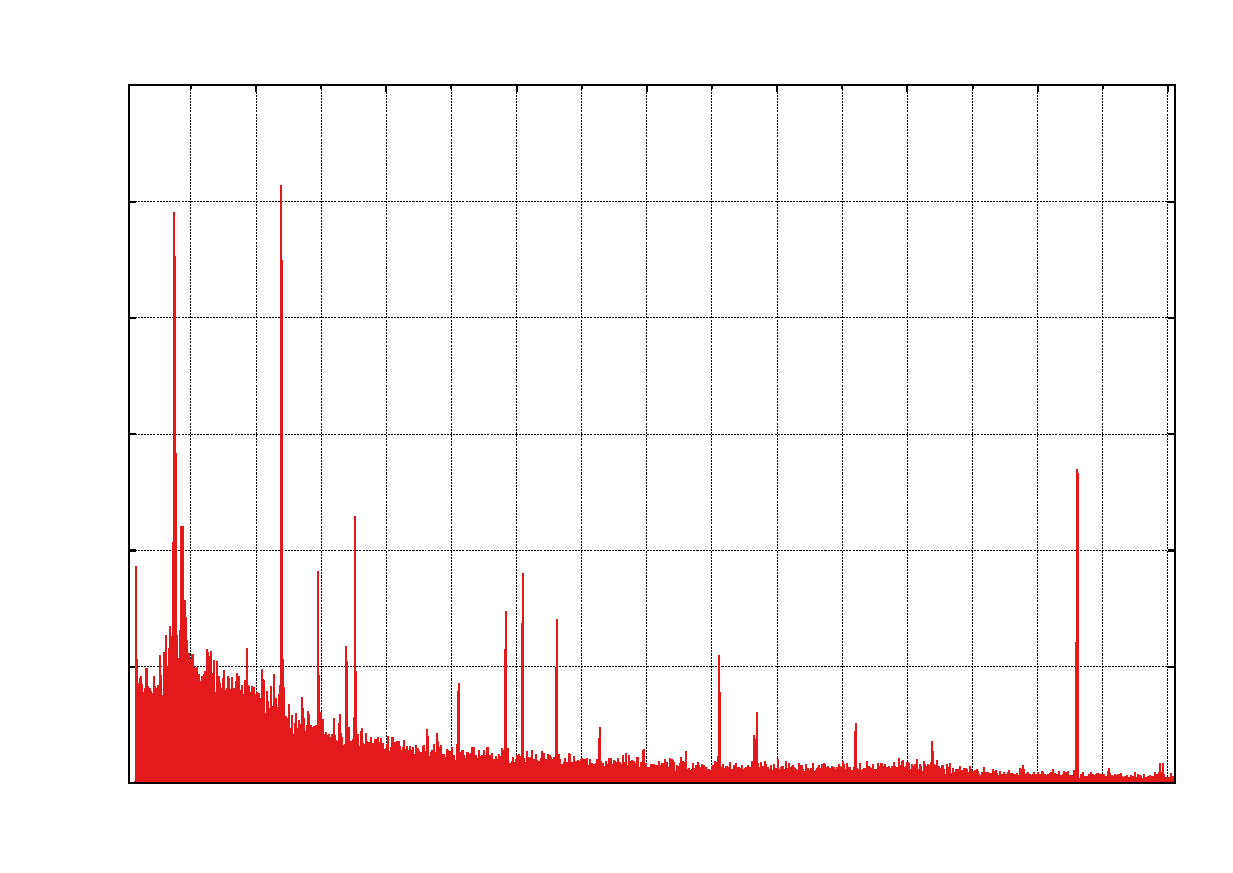
\includegraphics{./plots/langzeitmessung/probe_gross}}%
    \gplfronttext
  \end{picture}%
\endgroup

		\caption{Aufgenommenes Gammaspektrum der Bodenprobe mit nummerierten Peaks. Die zugehörigen Energien sind in Tabelle \ref{tab:langzeitmessung_linien} notiert.}
		\label{fig:langzeit_gross}
\end{sidewaysfigure}

\end{appendix}

\end{document}
